\documentclass[11pt,a4paper]{article}
\usepackage[utf8]{inputenc}
\usepackage[T1]{fontenc}
\usepackage[english]{babel}
\usepackage{geometry}
\usepackage{booktabs}
\usepackage{longtable}
\usepackage{array}
\usepackage{xcolor}
\usepackage{colortbl}
\usepackage{graphicx}
\usepackage{float}
\usepackage{subcaption}
\usepackage{fancyhdr}
\usepackage{titlesec}
\usepackage{tikz}
\usepackage{enumitem}
\usepackage{hyperref}
\usepackage{multicol}
\usepackage{listings}
\usepackage{tcolorbox}
\usepackage{amssymb}
\usepackage{amsmath}  


\geometry{margin=2cm}
\pagestyle{fancy}
\fancyhf{}
\rhead{Machine Learning Workshop}
\lhead{Customer Behavioral Analysis}
\rfoot{Page \thepage}

% Custom Colors
\definecolor{headerblue}{RGB}{41, 65, 114}
\definecolor{lightgray}{RGB}{245, 245, 245}
\definecolor{accentorange}{RGB}{230, 126, 34}
\definecolor{codegreen}{RGB}{0,128,0}
\definecolor{codegray}{RGB}{128,128,128}
\definecolor{codepurple}{RGB}{128,0,128}
\definecolor{backcolour}{RGB}{248,248,248}
\definecolor{warningred}{RGB}{231, 76, 60}
\definecolor{successgreen}{RGB}{46, 204, 113}

\lstdefinestyle{mystyle}{
    backgroundcolor=\color{backcolour},   
    commentstyle=\color{codegreen},
    keywordstyle=\color{codepurple},
    numberstyle=\tiny\color{codegray},
    stringstyle=\color{codegreen},
    basicstyle=\ttfamily\footnotesize,
    breakatwhitespace=false,         
    breaklines=true,                 
    captionpos=b,                    
    keepspaces=true,                 
    numbers=left,                    
    numbersep=5pt,                  
    showspaces=false,                
    showstringspaces=false,
    showtabs=false,                  
    tabsize=2
}
\lstset{style=mystyle}


\tcbset{
    colback=backcolour,
    colframe=headerblue,
    fonttitle=\bfseries,
    boxrule=1pt,
    arc=3mm
}


\titleformat{\section}
{\color{headerblue}\normalfont\Large\bfseries}
{\thesection}{1em}{}[{\titlerule[2pt]}]

\titleformat{\subsection}
{\color{accentorange}\normalfont\large\bfseries}
{\thesubsection}{1em}{}

% Custom column definitions
\newcolumntype{C}[1]{>{\centering\arraybackslash}p{#1}}
\newcolumntype{L}[1]{>{\raggedright\arraybackslash}p{#1}}

\begin{document}


\begin{titlepage}
\begin{tikzpicture}[remember picture,overlay]
    \fill[headerblue] (current page.north west) rectangle ([yshift=-5cm]current page.north east);
    \node[anchor=north west, xshift=2cm, yshift=-2cm, text=white] at (current page.north west) 
        {\Huge\textbf{Machine Learning Workshop}};
    \node[anchor=north west, xshift=2cm, yshift=-3.5cm, text=white] at (current page.north west) 
        {\Large\textit{Retail Customer Behavioral Analysis}};
\end{tikzpicture}

\vspace{6cm}

\begin{center}
{\LARGE\textbf{PROJECT REPORT}}\par
\vspace{1cm}
{\large Practical Workshop: Gift E-commerce}\par
\vspace{2cm}
{\large \textbf{Prepared by Hichem Hamza}}
\vspace{3cm}


\begin{tikzpicture}
    \draw[headerblue, line width=2pt] (0,0) -- (10,0);
\end{tikzpicture}

\vspace{2cm}



\vspace{5cm}

{\textbf{Academic Year: 2025-2026}}

\end{center}
\vfill
\end{titlepage}

\section{Introduction and Business Understanding}

In the context of an e-commerce company specializing in gifts, the primary objective of this project is to deeply understand customer behavior to personalize marketing strategies, reduce the churn rate, and optimize revenue. To achieve this, the project models customer activity and develops robust predictive frameworks guided strictly by the \textbf{CRISP-DM} methodology.

The business objectives technically translate to:
\begin{enumerate}
    \item A \textbf{multi-thematic segmentation} (exploratory, temporal, and frictional).
    \item A robust and interpretable \textbf{churn prediction} (binary classification).
    \item The \textbf{deployment} of these models via an interactive interface for operational teams.
\end{enumerate}

\section{Data Understanding}

The initial dataset includes over 4,300 customers and aggregates \textbf{52 variables (features)}. These variables offer a rich but complex view of user habits. A deep exploratory analysis (conducted via multiple Jupyter notebooks, e.g., \texttt{discover.ipynb}, \texttt{age\_impute.ipynb}, and validated in the production \texttt{preprocessing.py} script) identified several critical data quality challenges that dictate the preprocessing strategy.

\begin{tcolorbox}[title=Variable Typology \& Cardinality]
\begin{itemize}
    \item \textbf{Direct Behavioral Variables (Numerical)}: Recency, Frequency, Monetary (RFM), TotalQuantity.
    \item \textbf{Frictional Variables (Numerical)}: ReturnRatio, CancelledTransactions, SupportTicketsCount, SatisfactionScore.
    \item \textbf{Temporal Variables (Numerical \& Categorical)}: PreferredDayOfWeek, PreferredHour, WeekendPurchaseRatio.
    \item \textbf{Exploratory Variables (Numerical)}: UniqueProducts, UniqueCountries.
    \item \textbf{Categorical (Ordinal)}: Customer segments requiring algorithmic mapping, e.g., \textit{RFMSegment} (Dormants, Potentiels, Fidèles, Champions), \textit{AgeCategory} (18-24 to 65+), \textit{SpendingCategory} (Low, Medium, High, VIP), \textit{LoyaltyLevel}.
    \item \textbf{Categorical (Nominal)}: Variables requiring One-Hot Encoding, e.g., \textit{CustomerType}, \textit{FavoriteSeason}, \textit{Region}, \textit{Gender}, \textit{AccountStatus}.
\end{itemize}
\end{tcolorbox}

\subsection{Data Quality Anomalies and Missing Values}
The Exploratory Data Analysis phase uncovered several distinct patterns of missing or corrupted data:
\begin{itemize}
    \item \textbf{Missing Values Pattern}: The \textit{Age} feature suffers from approximately 30\% missing values. Other columns with extremely high NaN ratios ($>50\%$) were flagged for systemic removal.
    \item \textbf{Sentinel Values}: Dummy values were used natively in the dataset to represent null states. For example, \textit{SupportTicketsCount} contained \texttt{-1} and \texttt{999}. \textit{SatisfactionScore} contained \texttt{-1}, \texttt{0}, and \texttt{99}. Textual sentinels like \texttt{"Unknown"} or \texttt{"Unspecified"} were systematically identified in \textit{GeoIP} and \textit{Gender}.
    \item \textbf{Outliers}: Extreme deviations were identified requiring bounding (e.g., highly abnormal ticket counts or monetary returns, clipped at the 1st/99th percentiles or dropped if beyond the 5\% bounds in the isolation script).
\end{itemize}

\subsection{Feature Redundancy and Target Leakage}
A fundamental step in data understanding and preparation is preventing the model from learning tautologies or failing due to multicollinearity. This was handled extensively in our preprocessing pipeline (\texttt{src/preprocessing.py}) across two distinct phases.

\subsubsection{Structural Leakage Prevention}
Before any complex algorithm was applied, several variables were definitively pruned due to intrinsic logic derived during Exploratory Data Analysis:

\begin{itemize}
    \item \textbf{Non-Predictive Identifiers}: Fields such as \textit{CustomerID} and \textit{LastLoginIP} were removed as they provide zero generalized predictive value.
    \item \textbf{Zero Variance}: The \textit{NewsletterSubscribed} feature was found to be 100\% constant across all rows, offering absolutely zero informational entropy matrix-wise. Any feature exhibiting such variance collapse is aggressively dropped.
    \item \textbf{Target Leakage (\textit{ChurnRiskCategory})}: As demonstrated in \texttt{discover.ipynb}, the \textit{ChurnRiskCategory} variable strongly correlates with the target \textit{Churn} (near 0.9 correlation). This indicates it is likely a prediction made by an existing model or team, rather than raw behavioral data that can be organically gathered from a user's website activity. Retaining this field would constitute severe target leakage, artificially inflating model performance while being useless for predicting churn on genuinely new, unannotated profiles. It was thus permanently removed.
    \item \textbf{Target Leakage (\textit{Recency} \& Derivatives)}: \textit{Recency} heavily correlated with churn (since churners naturally stopped buying) and contained missing values structurally aligned with the churn event. It was systematically dropped. Furthermore, any engineered features explicitly dependent on it (such as the originally planned \textit{TenureRatio}) were deeply purged from the preprocessing scripts (\texttt{features.py}) to safely prevent secondary target leakage.
    \item \textbf{Target Leakage (\textit{RFMSegment})}: The \textit{RFMSegment} feature was additionally removed because it inherently relies on recency and frequency, functioning as a deterministic proxy for churn. Retaining it would create problematic data leakage when evaluating genuine independent behavioral signals.
    \item \textbf{Target Leakage (\textit{CustomerType})}: A devastating 100\% deterministic target leakage was discovered embedded within the \textit{CustomerType} variable. Cross-referencing exposed that the category ``Perdu'' (Lost) mapped exclusively to churned customers (Churn=1), while all active tags (``Occasionnel'', ``Régulier'', ``Hyperactif'') mapped flawlessly to active customers (Churn=0). Retaining this single feature allowed the models to artificially breach 99.7\% accuracy without genuinely learning churn behavior. It was entirely purged from the feature schema.
\end{itemize}

\subsubsection{Algorithmic Feature Selection (Post-Scaling)}
Beyond manual rules, dynamic feature selection layers the pipeline right before PCA projection to actively combat mathematical redundancy. These filters operate exclusively on the training set:

\begin{itemize}
    \item \textbf{Identifying Redundant Features}: Using \texttt{identify\_redundant\_features}, the correlation matrix is scanned dynamically. Any non-target variables strongly correlated with \textit{each other} are isolated to prevent multicollinearity, enforcing orthogonal learning. In the final pipeline run, exactly \textbf{16 features} were algorithmically dropped due to high redundancy (e.g., \textit{TotalQuantity}, \textit{TotalTransactions}, \textit{UniqueProducts}, and \textit{RegistrationYear}).
    \item \textbf{Mutual Information Pruning}: Through \texttt{identify\_non\_contributory\_features}, the pipeline formally evaluates the Mutual Information score of each surviving component against the discrete \textit{Churn} target. Any element falling below the $0.01$ significance threshold is classified as non-contributory noise and formally dropped. Combined with the redundancy filter, a total of \textbf{28 features} were dynamically pruned (including \textit{MonetaryAvg}, \textit{AvgQuantityPerTransaction}, and \textit{SupportTicketsCount}).
\end{itemize}

\section{Data Preparation}

This phase, crucial in the CRISP-DM approach, required rigorous preprocessing to avoid any data leakage between the training and testing sets.

\subsection{Pipeline Architecture and Leakage Prevention}
The cornerstone of this pipeline is a strict two-phase transformation architecture implemented via \texttt{fit\_transform\_train} and \texttt{transform\_test} functions. This separation is mandatory to prevent \textbf{data leakage}, where test-set statistics inadvertently contaminate the training process and inflate reported performance.

\begin{itemize}
    \item \textbf{Training phase} (\texttt{fit\_transform\_train}): All transformation parameters are \textit{learned exclusively} from the training data using \texttt{fit\_transform}. This includes the temporal reference date, target encoders, the KNN imputer, both scalers, the one-hot column schema, and the PCA projection matrix. The pruning lists for high-NaN and low-information features are also computed here.
    \item \textbf{Test phase} (\texttt{transform\_test}): The test set is processed using only a \texttt{transform} call — precisely applying the already-fitted artifacts with zero recalculation. No statistic from the test set influences any step.
    \item \textbf{Inference phase (deployment)}: The same \texttt{fitted\_artifacts.joblib} file is loaded by the Flask application at runtime. An incoming customer record is passed through the exact same sequenced pipeline, guaranteeing identical transformations.
\end{itemize}

The ten artifacts serialized to \texttt{fitted\_artifacts.joblib} are: \texttt{reference\_date}, \texttt{country\_enc}, \texttt{geoip\_enc}, \texttt{one\_hot\_columns}, \texttt{high\_nan\_cols}, \texttt{low\_nan\_cols}, \texttt{imputer}, \texttt{knn\_scaler}, \texttt{final\_scaler}, and \texttt{pca}.

\subsection{Cleaning and Feature Engineering}
The cleaning process was strictly partitioned to prevent any temporal or statistical data leakage. All transformation parameters (e.g., temporal reference dates, mean target likelihoods, imputation centroids) were derived exclusively from the separated training set. 

\begin{itemize}
    \item \textbf{Temporal Engineering}: The raw \textit{RegistrationDate} was transformed into the continuous quantitative feature \textit{DaysSinceRegistration}. Crucially, this was calculated by determining the \textbf{maximum} date (the most recent dataset snapshot) strictly within the training set, and computing the passing days from each customer's registration up to that global reference maximum. This eliminates ambiguity and anchors tenure securely.
    \item \textbf{Encoding Typologies}: Ordinal variables containing intrinsic semantic rank (e.g., \textit{LoyaltyLevel}) were explicitly mapped to numerical scales (1 to 4). To navigate high-cardinality boundaries without exploding the matrix dimensionality, \textit{Country} and \textit{GeoIP} underwent robust \textbf{Target Encoding} (with Bayesian smoothing factors of 30 and 20 respectively) mapped cleanly against the Churn label. Finally, standard \textbf{One-Hot Encoding} structured the remaining low-cardinality nominals (e.g., \textit{Gender}, \textit{Region}, \textit{CustomerType}).
\end{itemize}

\subsection{Mathematical Feature Engineering and Pruning}
To natively capture behavioral relativity rather than relying on raw totals, several additional features were engineered mathematically:
\begin{itemize}
    \item \textbf{AvgBasketValue}: $\frac{\text{MonetaryTotal}}{\text{Frequency}}$. Identifies the typical financial weight of each individual transaction.
    \item \textbf{TenureRatio}: $\frac{\text{Recency}}{\text{CustomerTenure}}$. Calculates the exact proportion of inactivity relative to the customer's total historical lifespan.
    \item \textbf{TicketIntensity}: $\frac{\text{SupportTicketsCount}}{\text{CustomerTenure} + 1}$. Evaluates operational friction normalized uniformly across time.
    \item \textbf{CancellationRate}: $\frac{\text{CancelledTrans}}{\text{Frequency}}$. Formally computes the failure rate of attempted orders per customer.
    \item \textbf{ZeroPriceRatio}: $\frac{\text{ZeroPriceCount}}{\text{TotalTrans}}$. Highlights the proportion of purely promotional or free items acquired relative to total engagement.
\end{itemize}

However, mere generation of features does not guarantee predictive value. Following missing value imputation and prior to PCA, a strict multidimensional filtering pipeline was enforced (Correlation $\ge$ 0.8, Variance Inflation Factor $\ge$ 10, and Mutual Information with Churn $< 0.01$). 
\textbf{Notably, the ``CancellationRate'' feature (despite being explicitly suggested in the preliminary project specifications)} was cleanly pruned by this empirical pipeline. Analytical scans revealed that it failed stringent independence tests; its informational variance was fundamentally non-contributory or completely redundant relative to preexisting metrics like \textit{ReturnRatio} and the target itself. Thus, it was programmatically dropped to protect the models from collinear noise.

\subsection{Missing Value Management and Outlier Isolation}
Instead of relying on a single uniform imputation approach, missing infrastructure was structurally triaged. Sentinel placeholders deeply embedded in the dataset (such as \texttt{-1} and \texttt{999} for \textit{SupportTicketsCount}, or \texttt{"Unspecified"} and \texttt{"Inconnu"} for textual features) were successfully programmatically reverted back to explicit \texttt{NaN} representations. 

Next, a strict thresholding test was parameterized: any feature missing more than 50\% of its entries in the training set was automatically pruned. Before proceeding to imputation on the surviving columns, \textbf{Outlier Filtering} systematically eliminated the extreme upper and lower 5\% bounds on highly erratic operational metrics like \textit{SupportTicketsCount} and \textit{SatisfactionScore} to prevent them from dramatically skewing spatial algorithms.

To illustrate the imputation strategy concretely, the \textit{Age} column is examined here: with 30\% of its values missing, a deliberate choice had to be made. Because the underlying distribution of the known ages was almost uniform rather than normally distributed, simple standard techniques such as mean or median imputation were explicitly rejected. Applying a median imputation would have artificially spiked the center of the distribution, creating severe statistical artifacts and destroying the natural variance required by the models. Instead, imputation was conducted using the K-Nearest Neighbors (\textbf{KNN Imputer}) algorithm. By evaluating adjacent customer profiles based on other behavioral features, KNN successfully recovered the missing ages while preserving the original structural variance without introducing major bias (see Figure~\ref{fig:age_imputation}).

\begin{figure}[H]
    \centering
    \begin{subfigure}{0.48\textwidth}
        \centering
        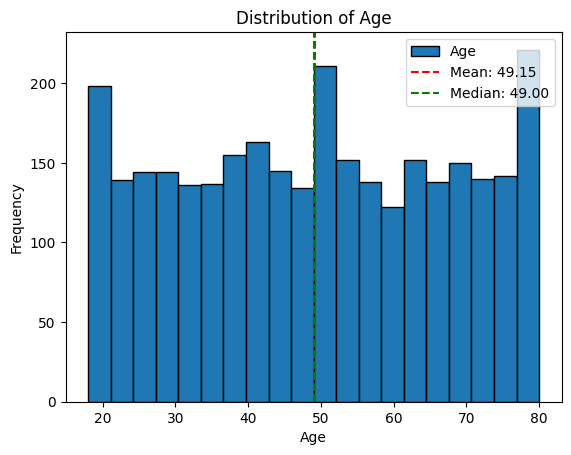
\includegraphics[width=\linewidth]{figures/eda/original_age_dist.png}
        \caption{Original Distribution}
    \end{subfigure}
    \hfill
    \begin{subfigure}{0.48\textwidth}
        \centering
        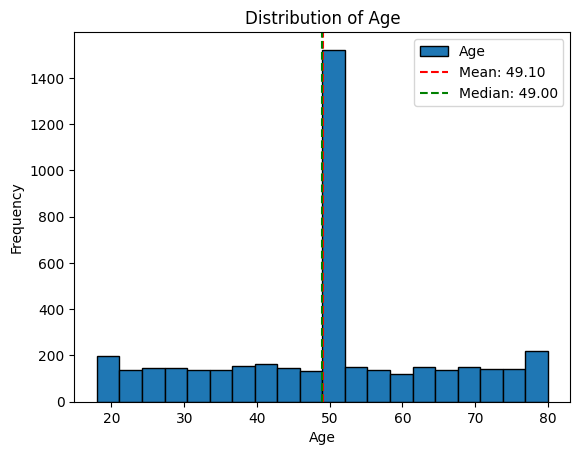
\includegraphics[width=\linewidth]{figures/eda/med_age_dist.png}
        \caption{Median Imputation Spike}
    \end{subfigure}
    
    \vspace{0.4cm}
    \begin{subfigure}{0.6\textwidth}
        \centering
        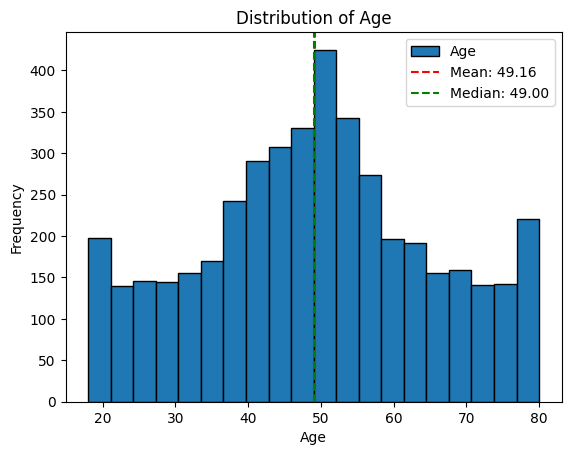
\includegraphics[width=\linewidth]{figures/eda/new_age_dist.png}
        \caption{KNN Imputation}
    \end{subfigure}
    \caption{Age Imputation Analysis: (a) shows the original almost uniform age distribution. (b) illustrates the severe artificial spike that median imputation would have caused. (c) demonstrates the final robust distribution achieved using the multidimensional KNN Imputer.}
    \label{fig:age_imputation}
\end{figure}

Following imputation, a rigorous feature selection layer dropped any surviving components that provided non-contributory mutual information relative to Churn (threshold $<$ 0.01) before standardizing scales.

\subsection{Standardization and Dimensionality Reduction}
To harmonize scales, all variables were standardized (mean of 0, standard deviation of 1) before applying Principal Component Analysis (\textbf{PCA}). The PCA preserved 99\% of the statistical variance by successfully compressing the transformed feature space down to exactly \textbf{31 principal components}. 
During algorithmic testing, a more aggressive 98\% variance threshold was evaluated. However, this threshold only marginally reduced the feature space to \textbf{29 components} (a minimal gain in dimensionality compression) while triggering a noticeable degradation in downstream classification performance. Consequently, the 99\% target was explicitly locked as the optimal structural anchor. While the full 31-dimensional space is strictly utilized by the predictive models to capture variance, a strictly 2-dimensional spatial projection (isolating just the first two principal components) is provided in \textbf{Figure~\ref{fig:pca}} to offer a human-readable visualization of the dataset's structural distribution.

\begin{figure}[H]
    \centering
    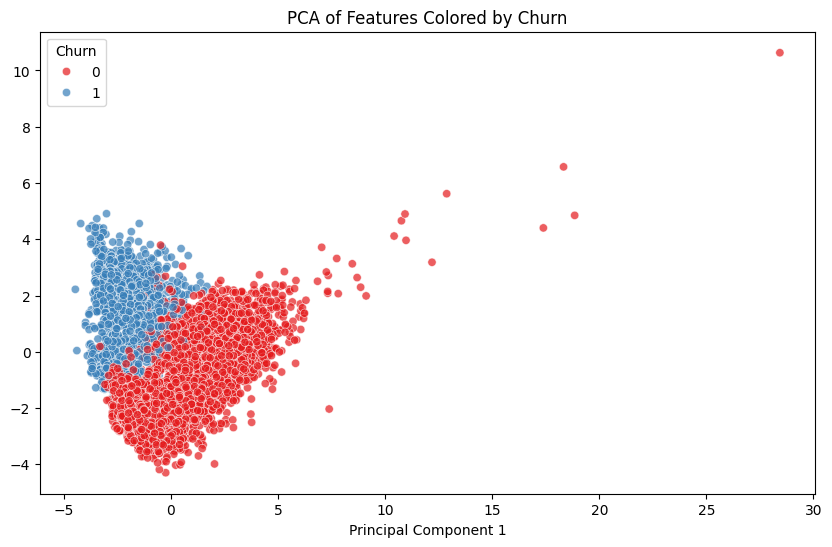
\includegraphics[width=0.6\textwidth]{figures/eda/PCA_2D.png}
    \caption{2D Principal Component Analysis visualizing the structural distribution.}
    \label{fig:pca}
\end{figure}

\subsection{Class Balancing}
To correct the severe imbalance of the \textit{Churn} target variable, the \textbf{SMOTE} (Synthetic Minority Oversampling Technique) oversampling method was applied exclusively to the training set, thus preserving the metric reality of the test set (Figure~\ref{fig:smote_balance}).

\begin{figure}[H]
    \centering
    \begin{subfigure}{0.48\textwidth}
        \centering
        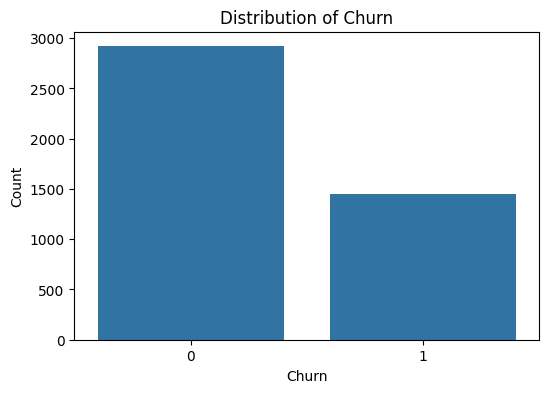
\includegraphics[width=\linewidth]{figures/eda/dist_before_balancing.png}
        \caption{Before SMOTE: severe class imbalance}
    \end{subfigure}
    \hfill
    \begin{subfigure}{0.48\textwidth}
        \centering
        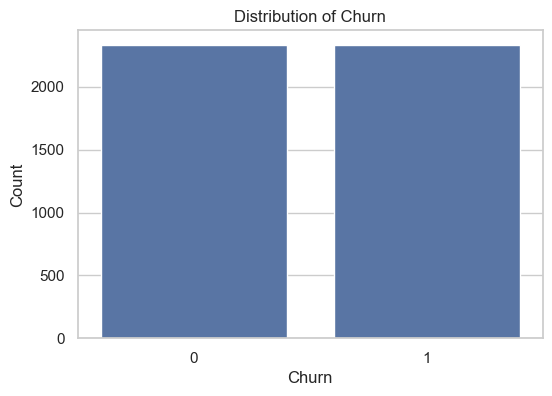
\includegraphics[width=\linewidth]{figures/eda/dist_after_balancing.png}
        \caption{After SMOTE: balanced target distribution}
    \end{subfigure}
    \caption{Class Distribution of the \textit{Churn} target variable before and after SMOTE oversampling applied exclusively to the training set.}
    \label{fig:smote_balance}
\end{figure}

\section{Modeling}

Modeling was conducted along two axes: unsupervised learning for segmentation and supervised learning for churn prediction.

\subsection{Multi-Thematic Segmentation (K-Means)}
Rather than applying the K-Means algorithm to a global and noisy point cloud, a three-part thematic approach was selected (Figure~\ref{fig:segment_profiles}):
\begin{itemize}
    \item \textbf{"Friction" Axis}: Analyzes operational cost (Support, returns, cancellations). Four clusters emerged: \textit{Low-Support, High-Support, Serial-Canceller, High-Returner}.
    \item \textbf{"Explorer" Axis}: Measures the breadth of catalog interactions. Clusters obtained: \textit{Focused-Buyer} and \textit{Broad-Explorer}.
    \item \textbf{"Timing" Axis}: Studies temporal cadence to extract \textit{Weekday-Shoppers} and \textit{Weekend-Shoppers}.
\end{itemize}

\begin{figure}[H]
    \centering
    \begin{subfigure}{0.48\textwidth}
        \centering
        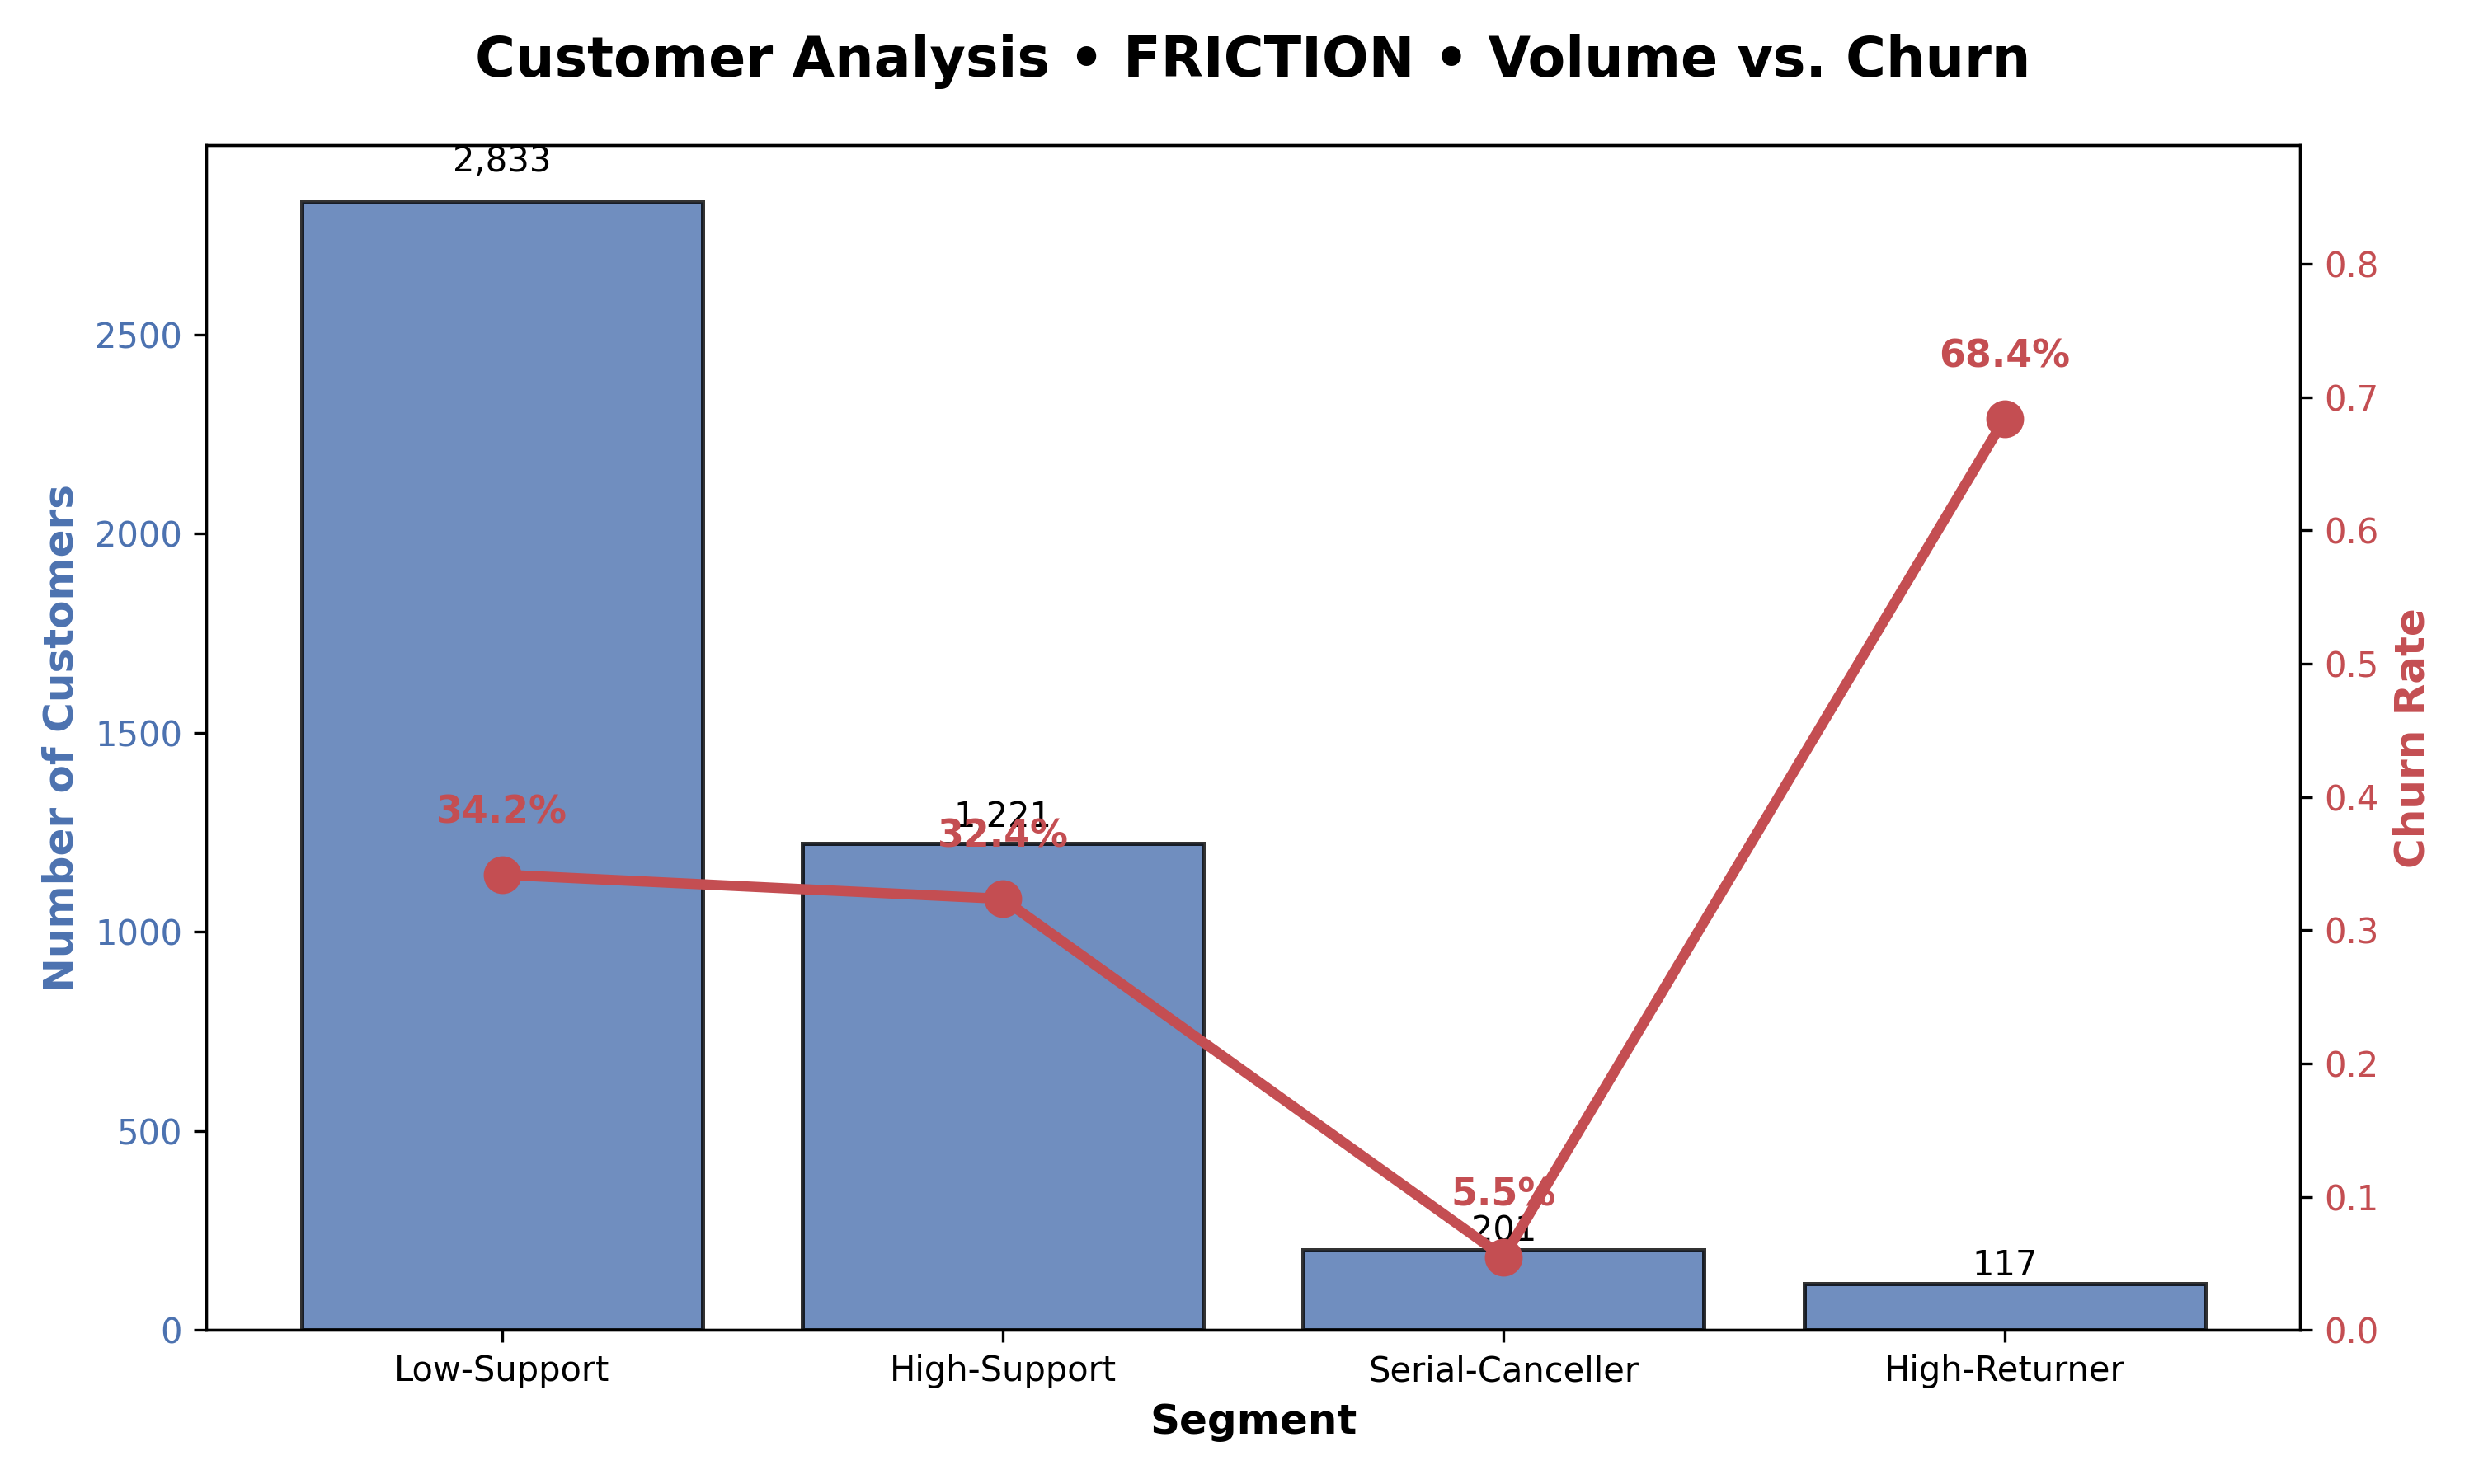
\includegraphics[width=\linewidth]{figures/segmentation/friction_size_vs_churn.png}
        \caption{Friction Axis Profile}
    \end{subfigure}
    \hfill
    \begin{subfigure}{0.48\textwidth}
        \centering
        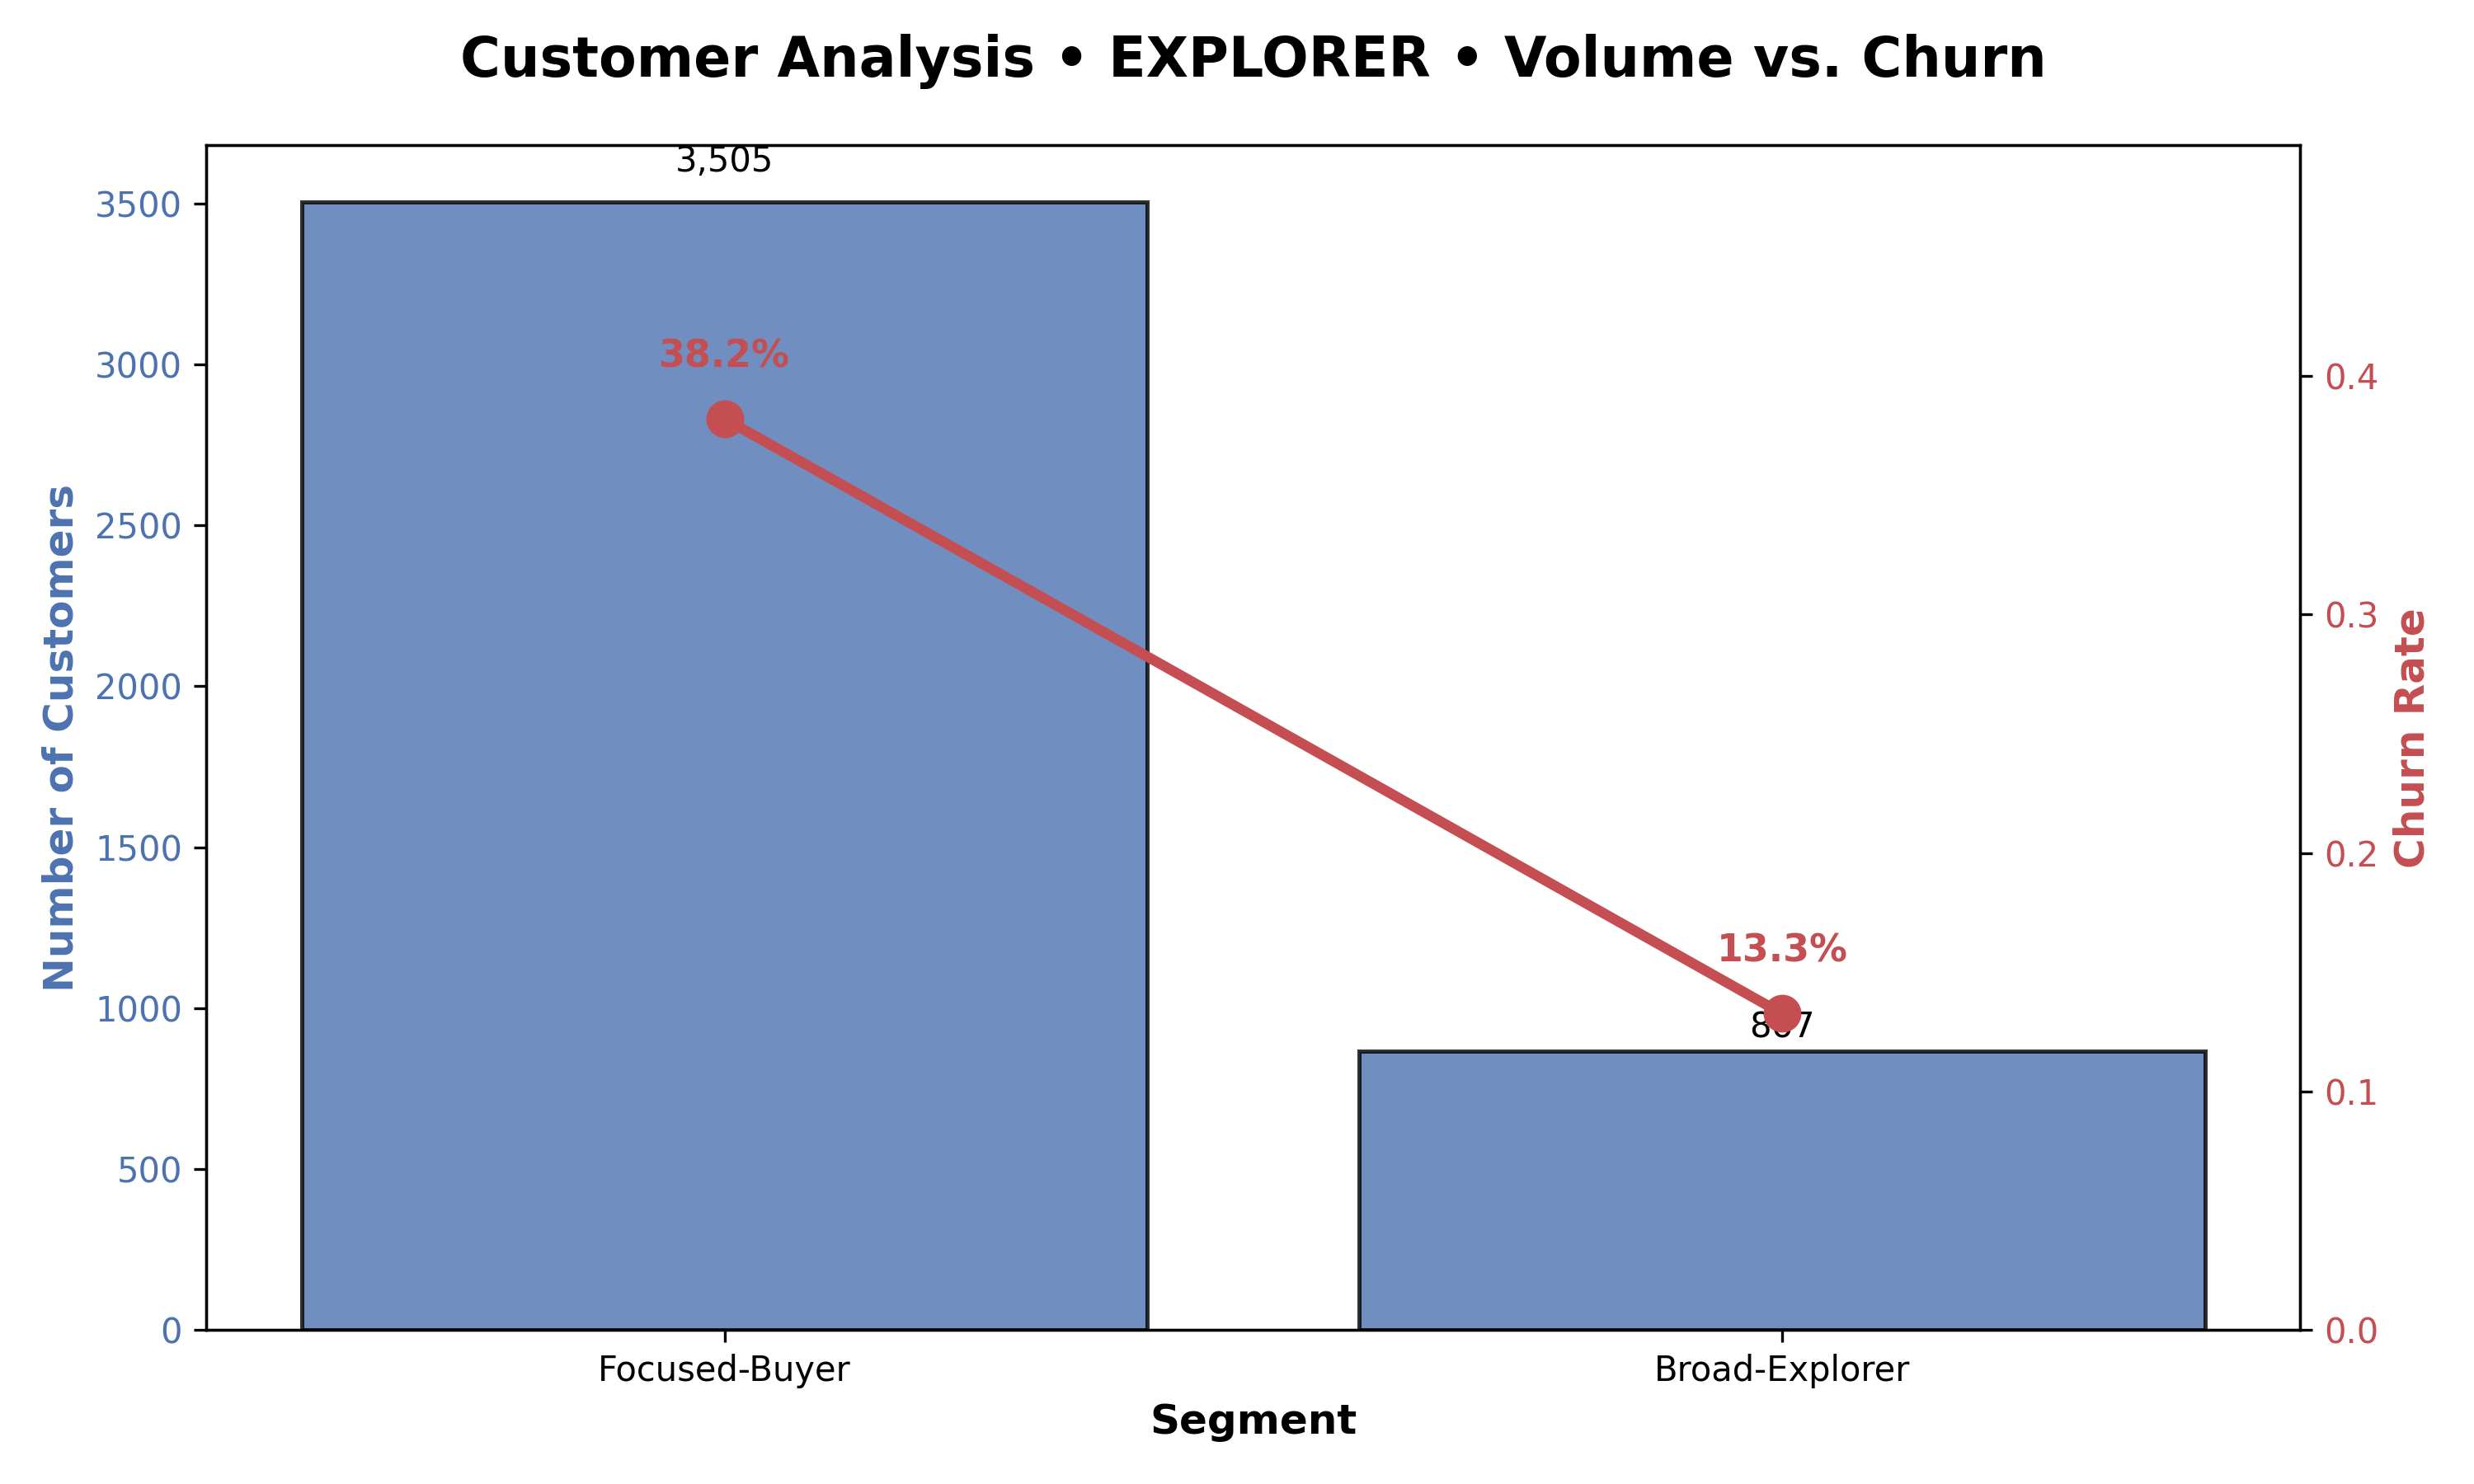
\includegraphics[width=\linewidth]{figures/segmentation/explorer_size_vs_churn.png}
        \caption{Explorer Axis Profile}
    \end{subfigure}
    \caption{Segment Profiles: Cluster sizes relative to Churn rates across different thematic axes.}
    \label{fig:segment_profiles}
\end{figure}

\subsection{Churn Prediction (Classification)}
We modeled the target variable across four formidable algorithms:
\begin{itemize}
    \item \textbf{Logistic Regression}: As a linear baseline reference.
    \item \textbf{Random Forest} and \textbf{Gradient Boosting}: Powerful ensemble methods for non-linear relationships.
    \item \textbf{XGBoost}: Specifically handles class imbalance via the \texttt{scale\_pos\_weight} parameter and captures predictive behaviors with high precision.
\end{itemize}
Hyperparameter tuning was optimized through \texttt{GridSearchCV} (3-fold Cross-Validation) by maximizing the area under the ROC curve.

\section{Evaluation}

The evaluation of the models' relevance validated the architectural choices from the previous phase.

\subsection{Segmentation Validation}
The generated segmentation reports quantitatively confirm the discriminative power of the thematic approach (see Figure~\ref{fig:segment_profiles}). Each axis produces clusters with meaningfully differentiated churn risk profiles, providing actionable granularity that a global single-run K-Means would obscure.

\textbf{Friction Axis} (Silhouette Score: 0.84 --- four clusters):
\begin{itemize}
    \item \textbf{Low-Support} (64.8\%, $n$=2{,}833): The largest cluster. Churn risk of 34.2\%. Silent customers who rarely contact support yet exhibit standard churn risk, making them difficult to detect proactively.
    \item \textbf{High-Support} (27.9\%, $n$=1{,}221): Churn risk of 32.4\%. Counter-intuitively, high support interaction correlates with slightly better retention, suggesting active engagement rather than dissatisfaction.
    \item \textbf{Serial-Canceller} (4.6\%, $n$=201): Churn risk of only 5.5\%. Despite high cancellation counts, these customers continue purchasing, suggesting systematic stock or fulfillment mismatches rather than intent to leave.
    \item \textbf{High-Returner} (2.7\%, $n$=117): The highest-risk cluster at \textbf{68.4\% churn}. A return rate near 40\% signals structural dissatisfaction, likely rooted in product description or quality expectations.
\end{itemize}

\textbf{Explorer Axis} (Silhouette Score: 0.59 --- two clusters):
\begin{itemize}
    \item \textbf{Focused-Buyer} (80.2\%, $n$=3{,}505): Churn risk of 38.2\%. Narrow purchase scope concentrated within specific product categories.
    \item \textbf{Broad-Explorer} (19.8\%, $n$=867): Churn risk of only \textbf{13.3\%} --- the most loyal cohort across all axes. Breadth of catalog engagement correlates strongly with retention.
\end{itemize}

\textbf{Timing Axis} (Silhouette Score: 0.41 --- two clusters):
\begin{itemize}
    \item \textbf{Weekday-Shopper} (86.8\%, $n$=3{,}797): Churn risk of 33.6\%. The dominant group with activity concentrated during the working week.
    \item \textbf{Weekend-Shopper} (13.2\%, $n$=575): Churn risk of 30.8\%. Marginally lower churn and clearly shifted purchase timing, suitable for targeted weekend-specific campaigns.
\end{itemize}

\begin{figure}[H]
    \centering
    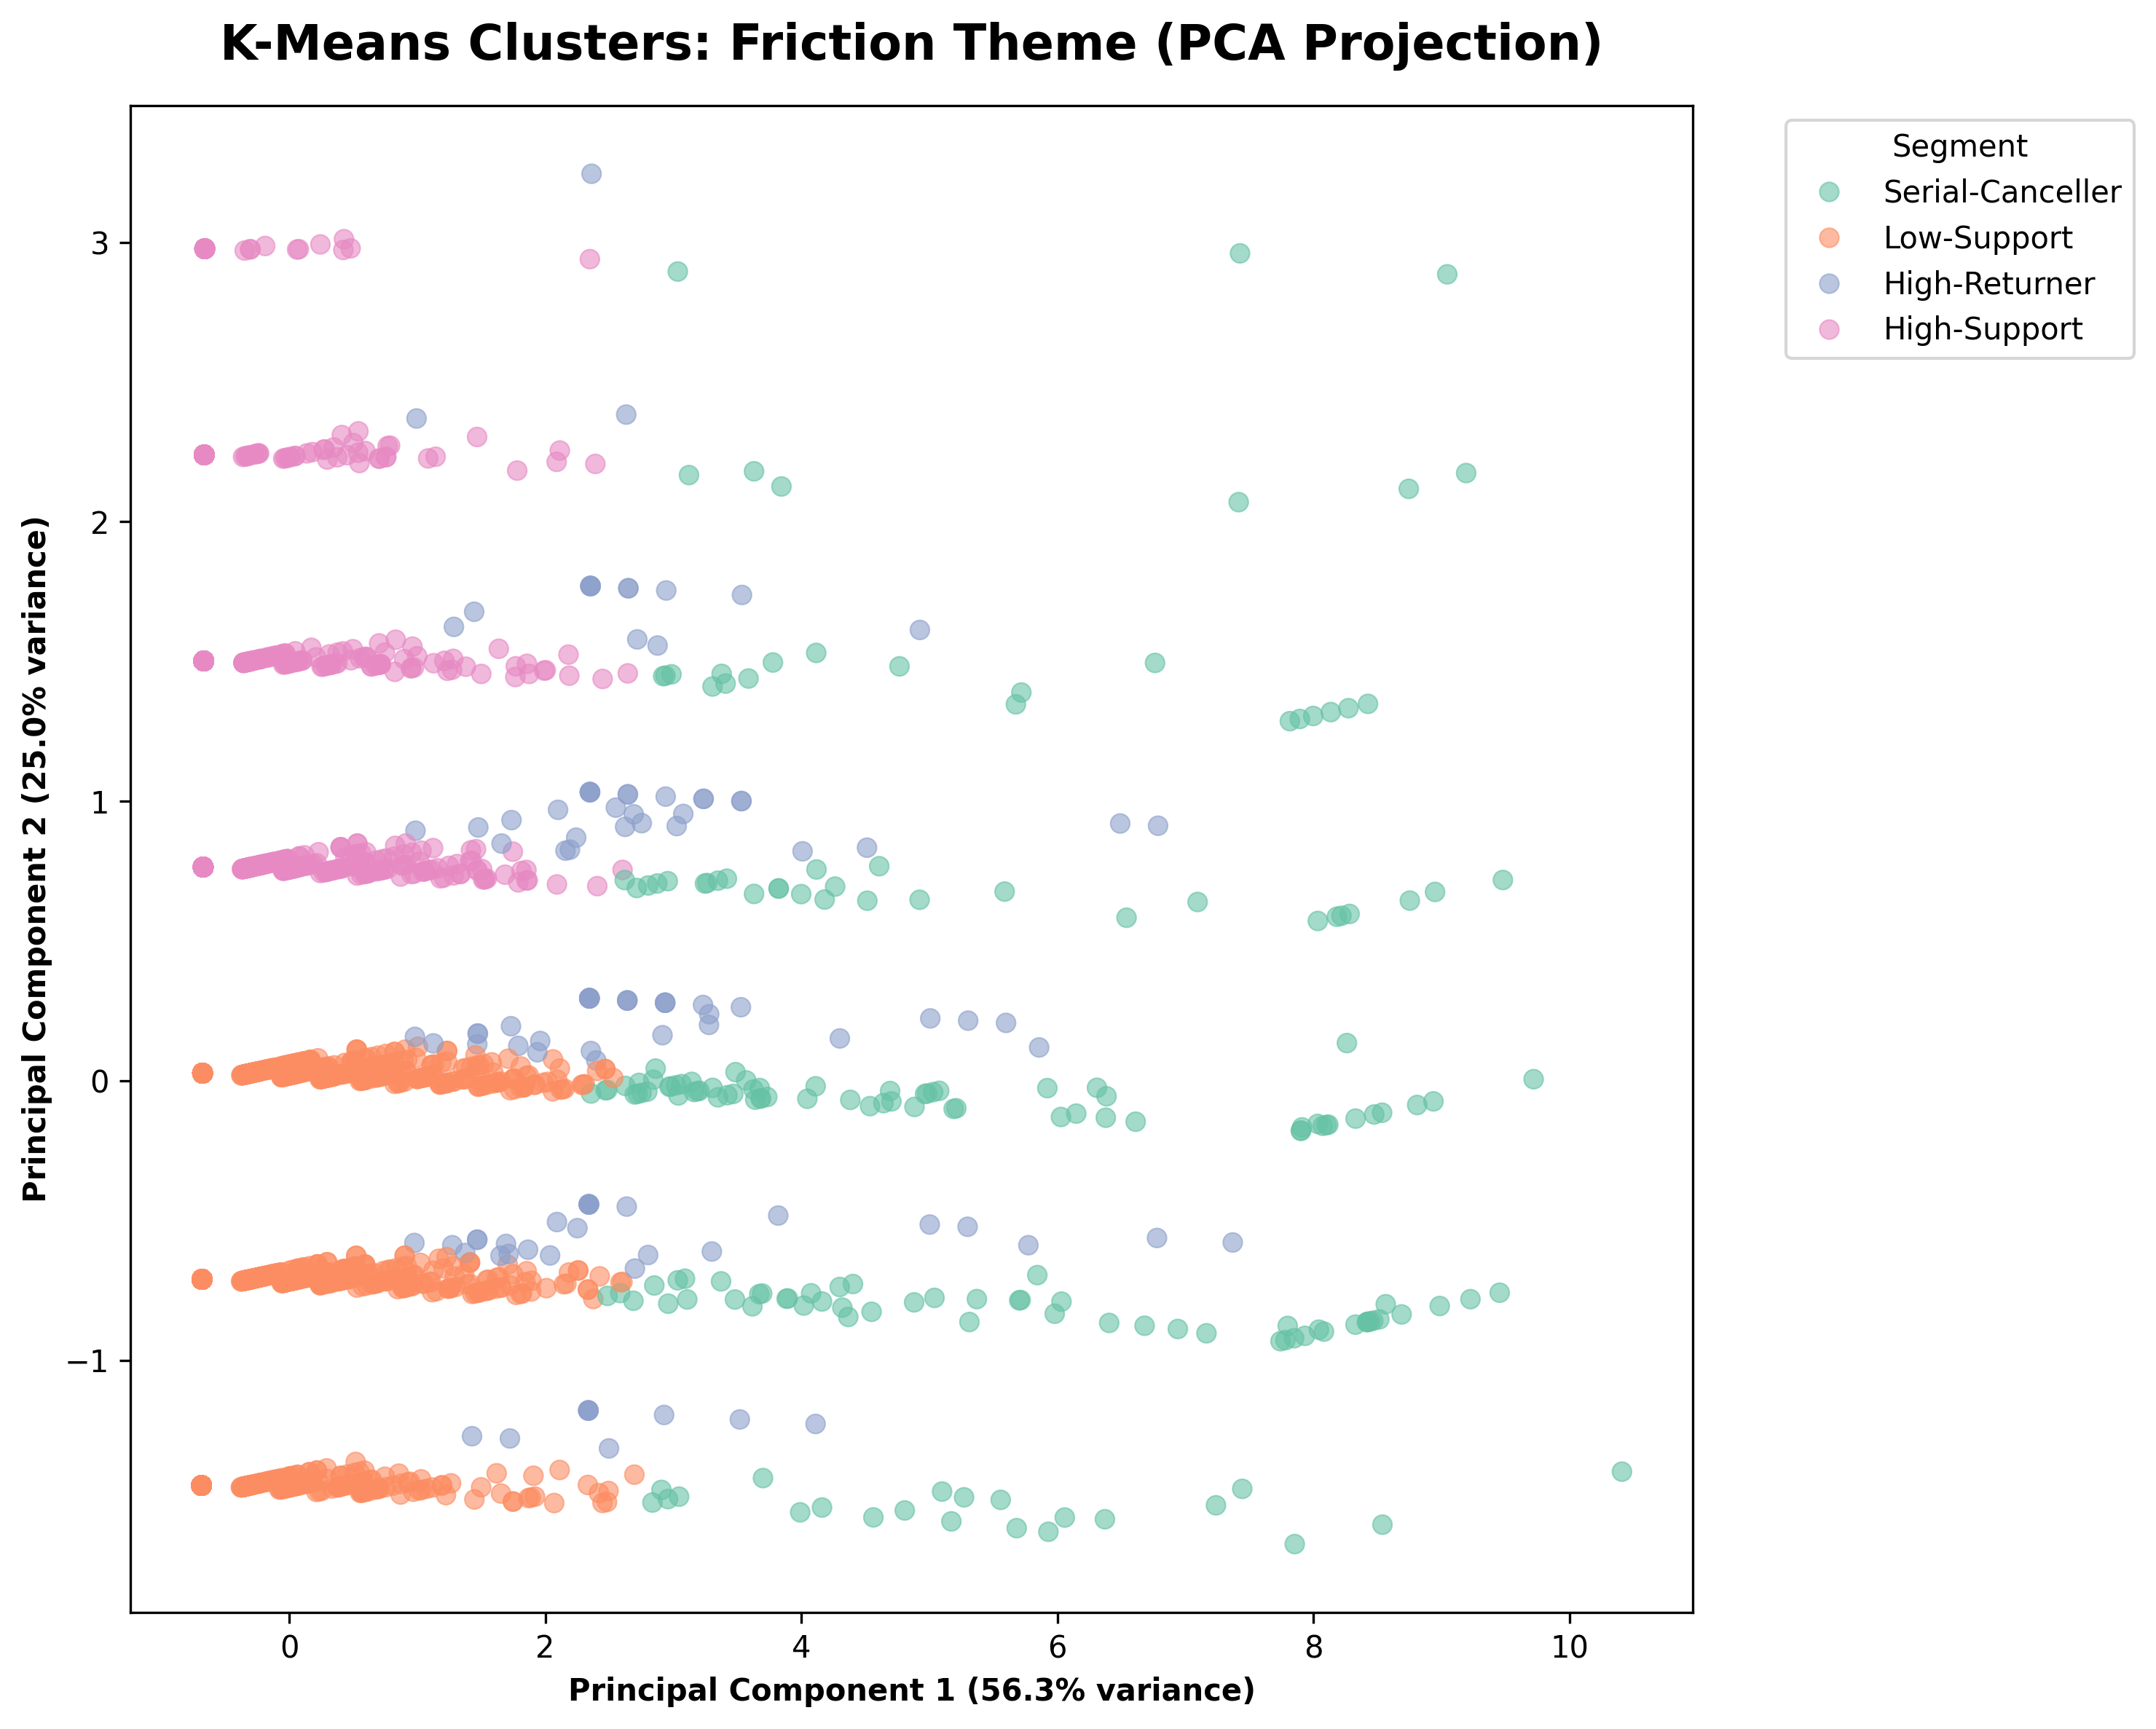
\includegraphics[width=0.9\textwidth]{figures/segmentation/friction_kmeans_scatter.png}
    \caption{Friction Axis --- Cluster scatter (PCA projection). Low-Support, High-Support, Serial-Canceller, High-Returner.}
    \label{fig:friction_seg}
\end{figure}

\begin{figure}[H]
    \centering
    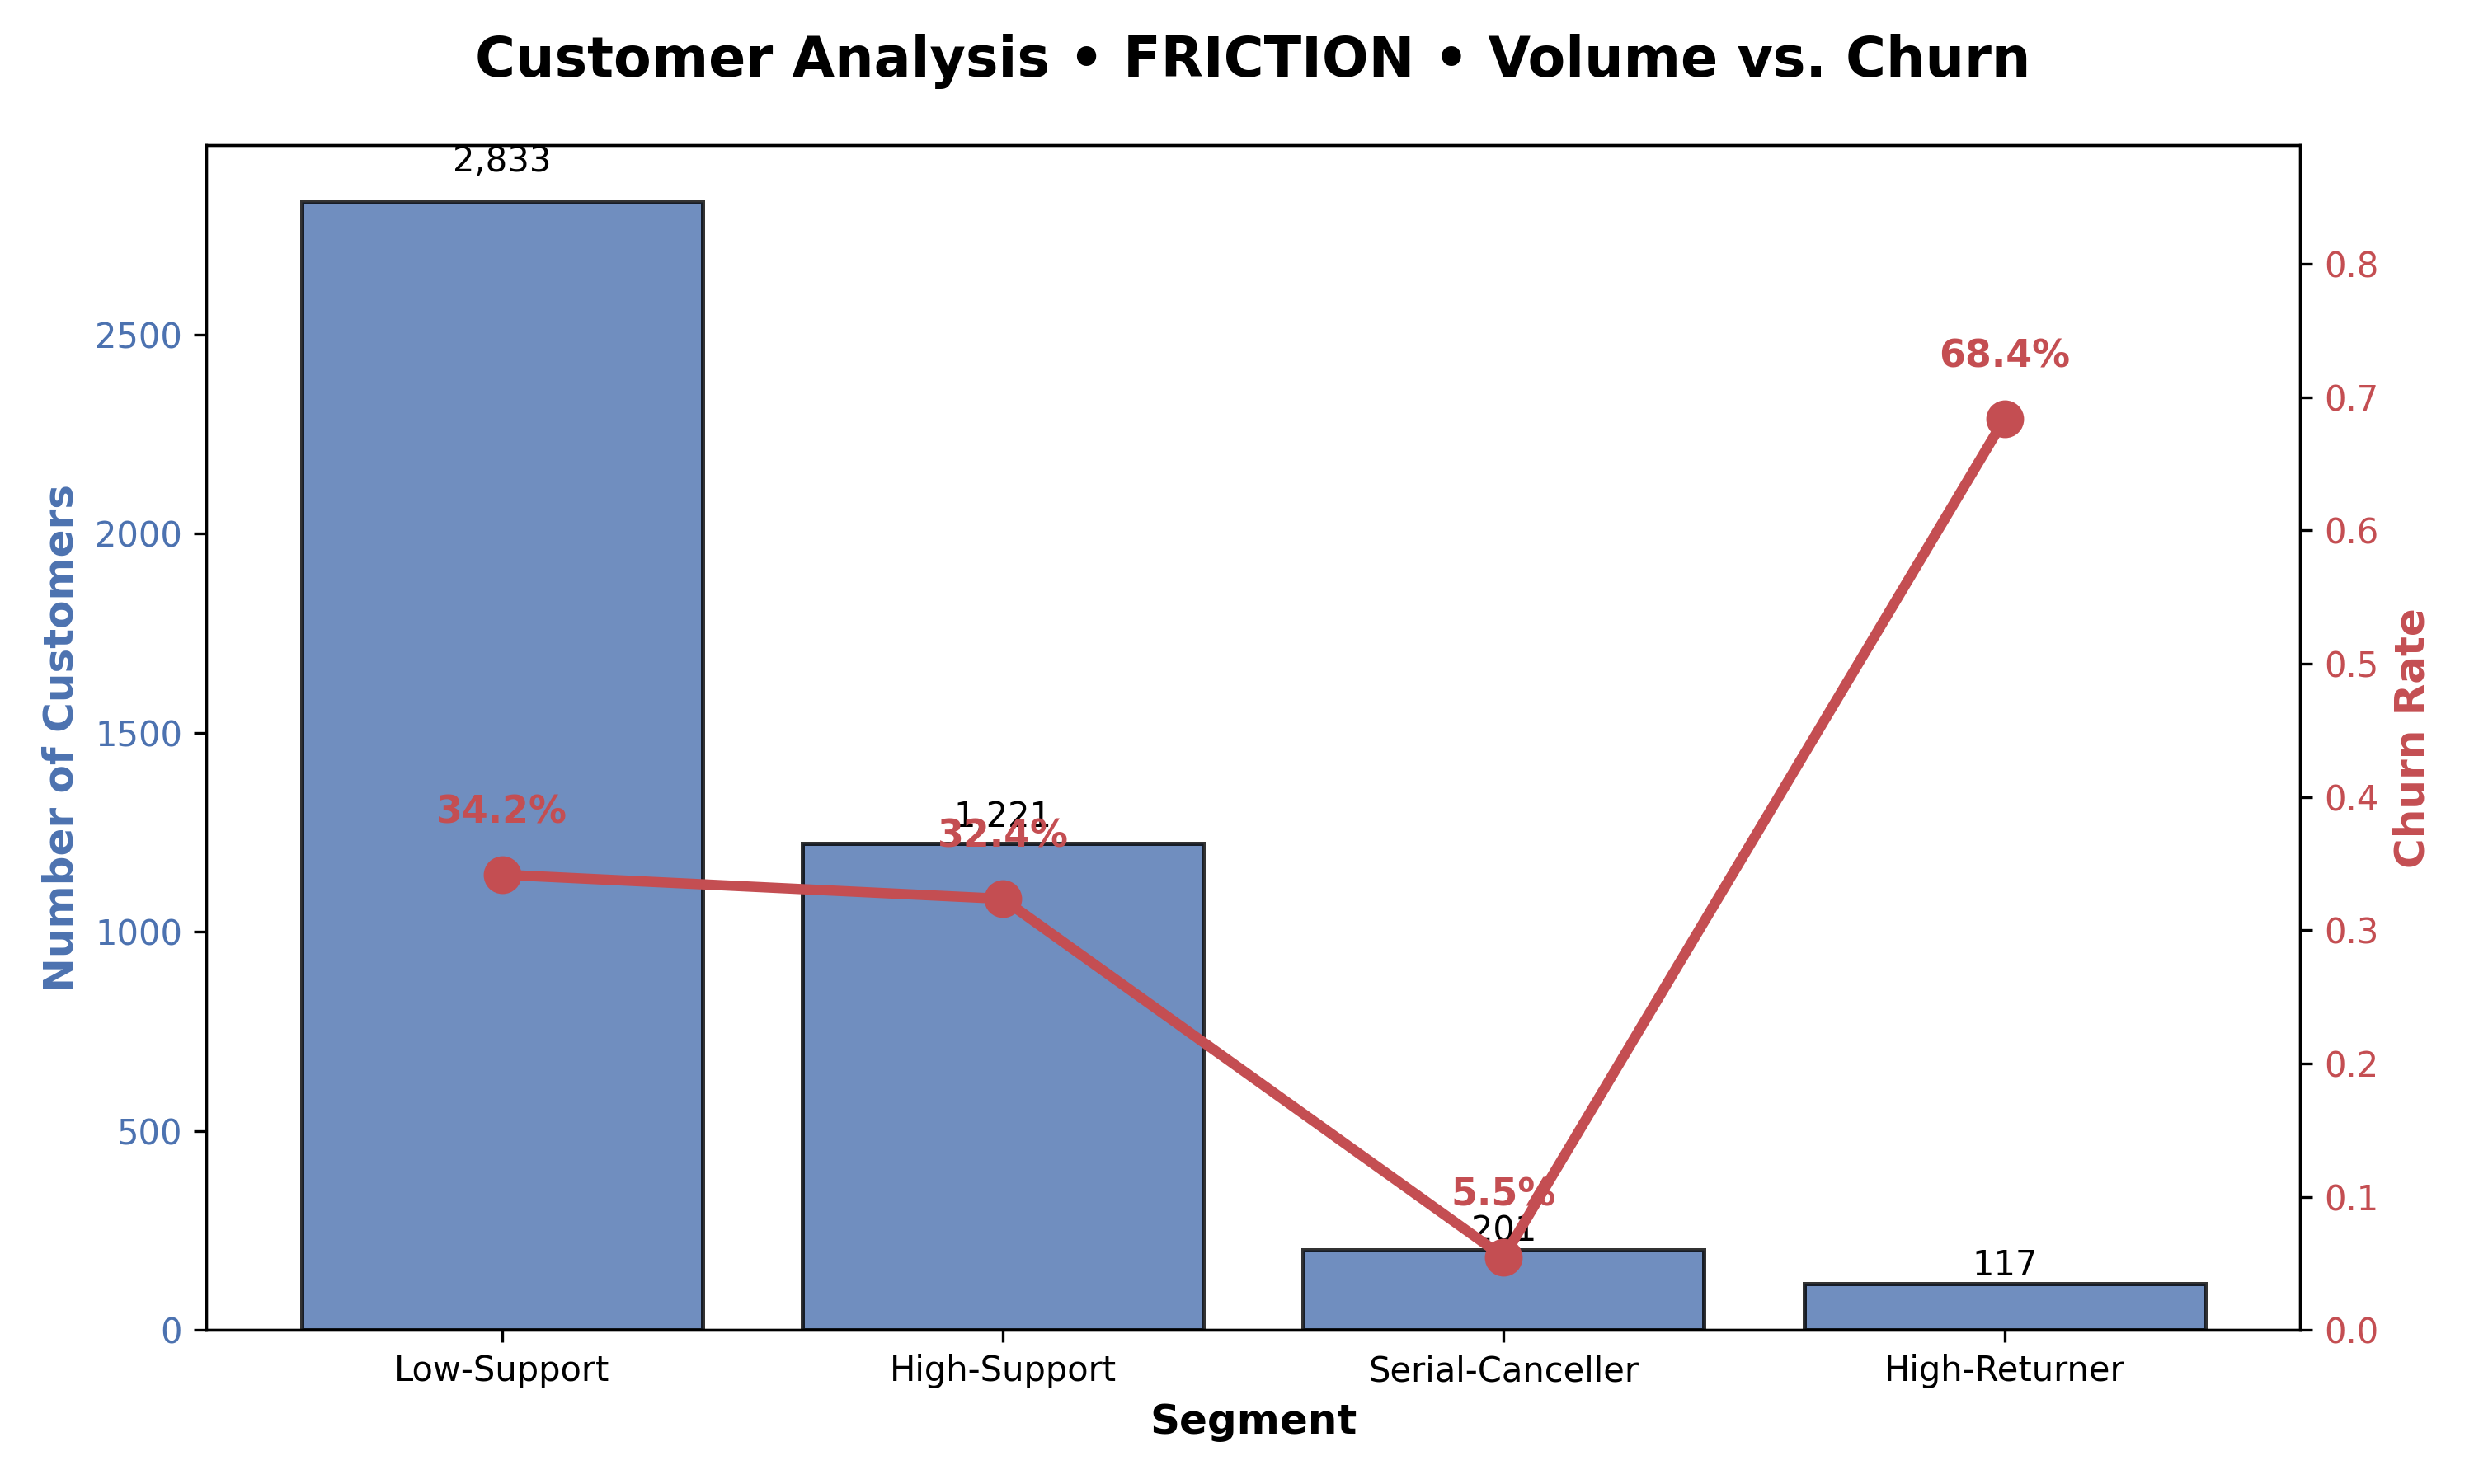
\includegraphics[width=0.75\textwidth]{figures/segmentation/friction_size_vs_churn.png}
    \caption{Friction Axis --- Cluster size vs. churn rate (Silhouette: 0.84).}
\end{figure}

\begin{figure}[H]
    \centering
    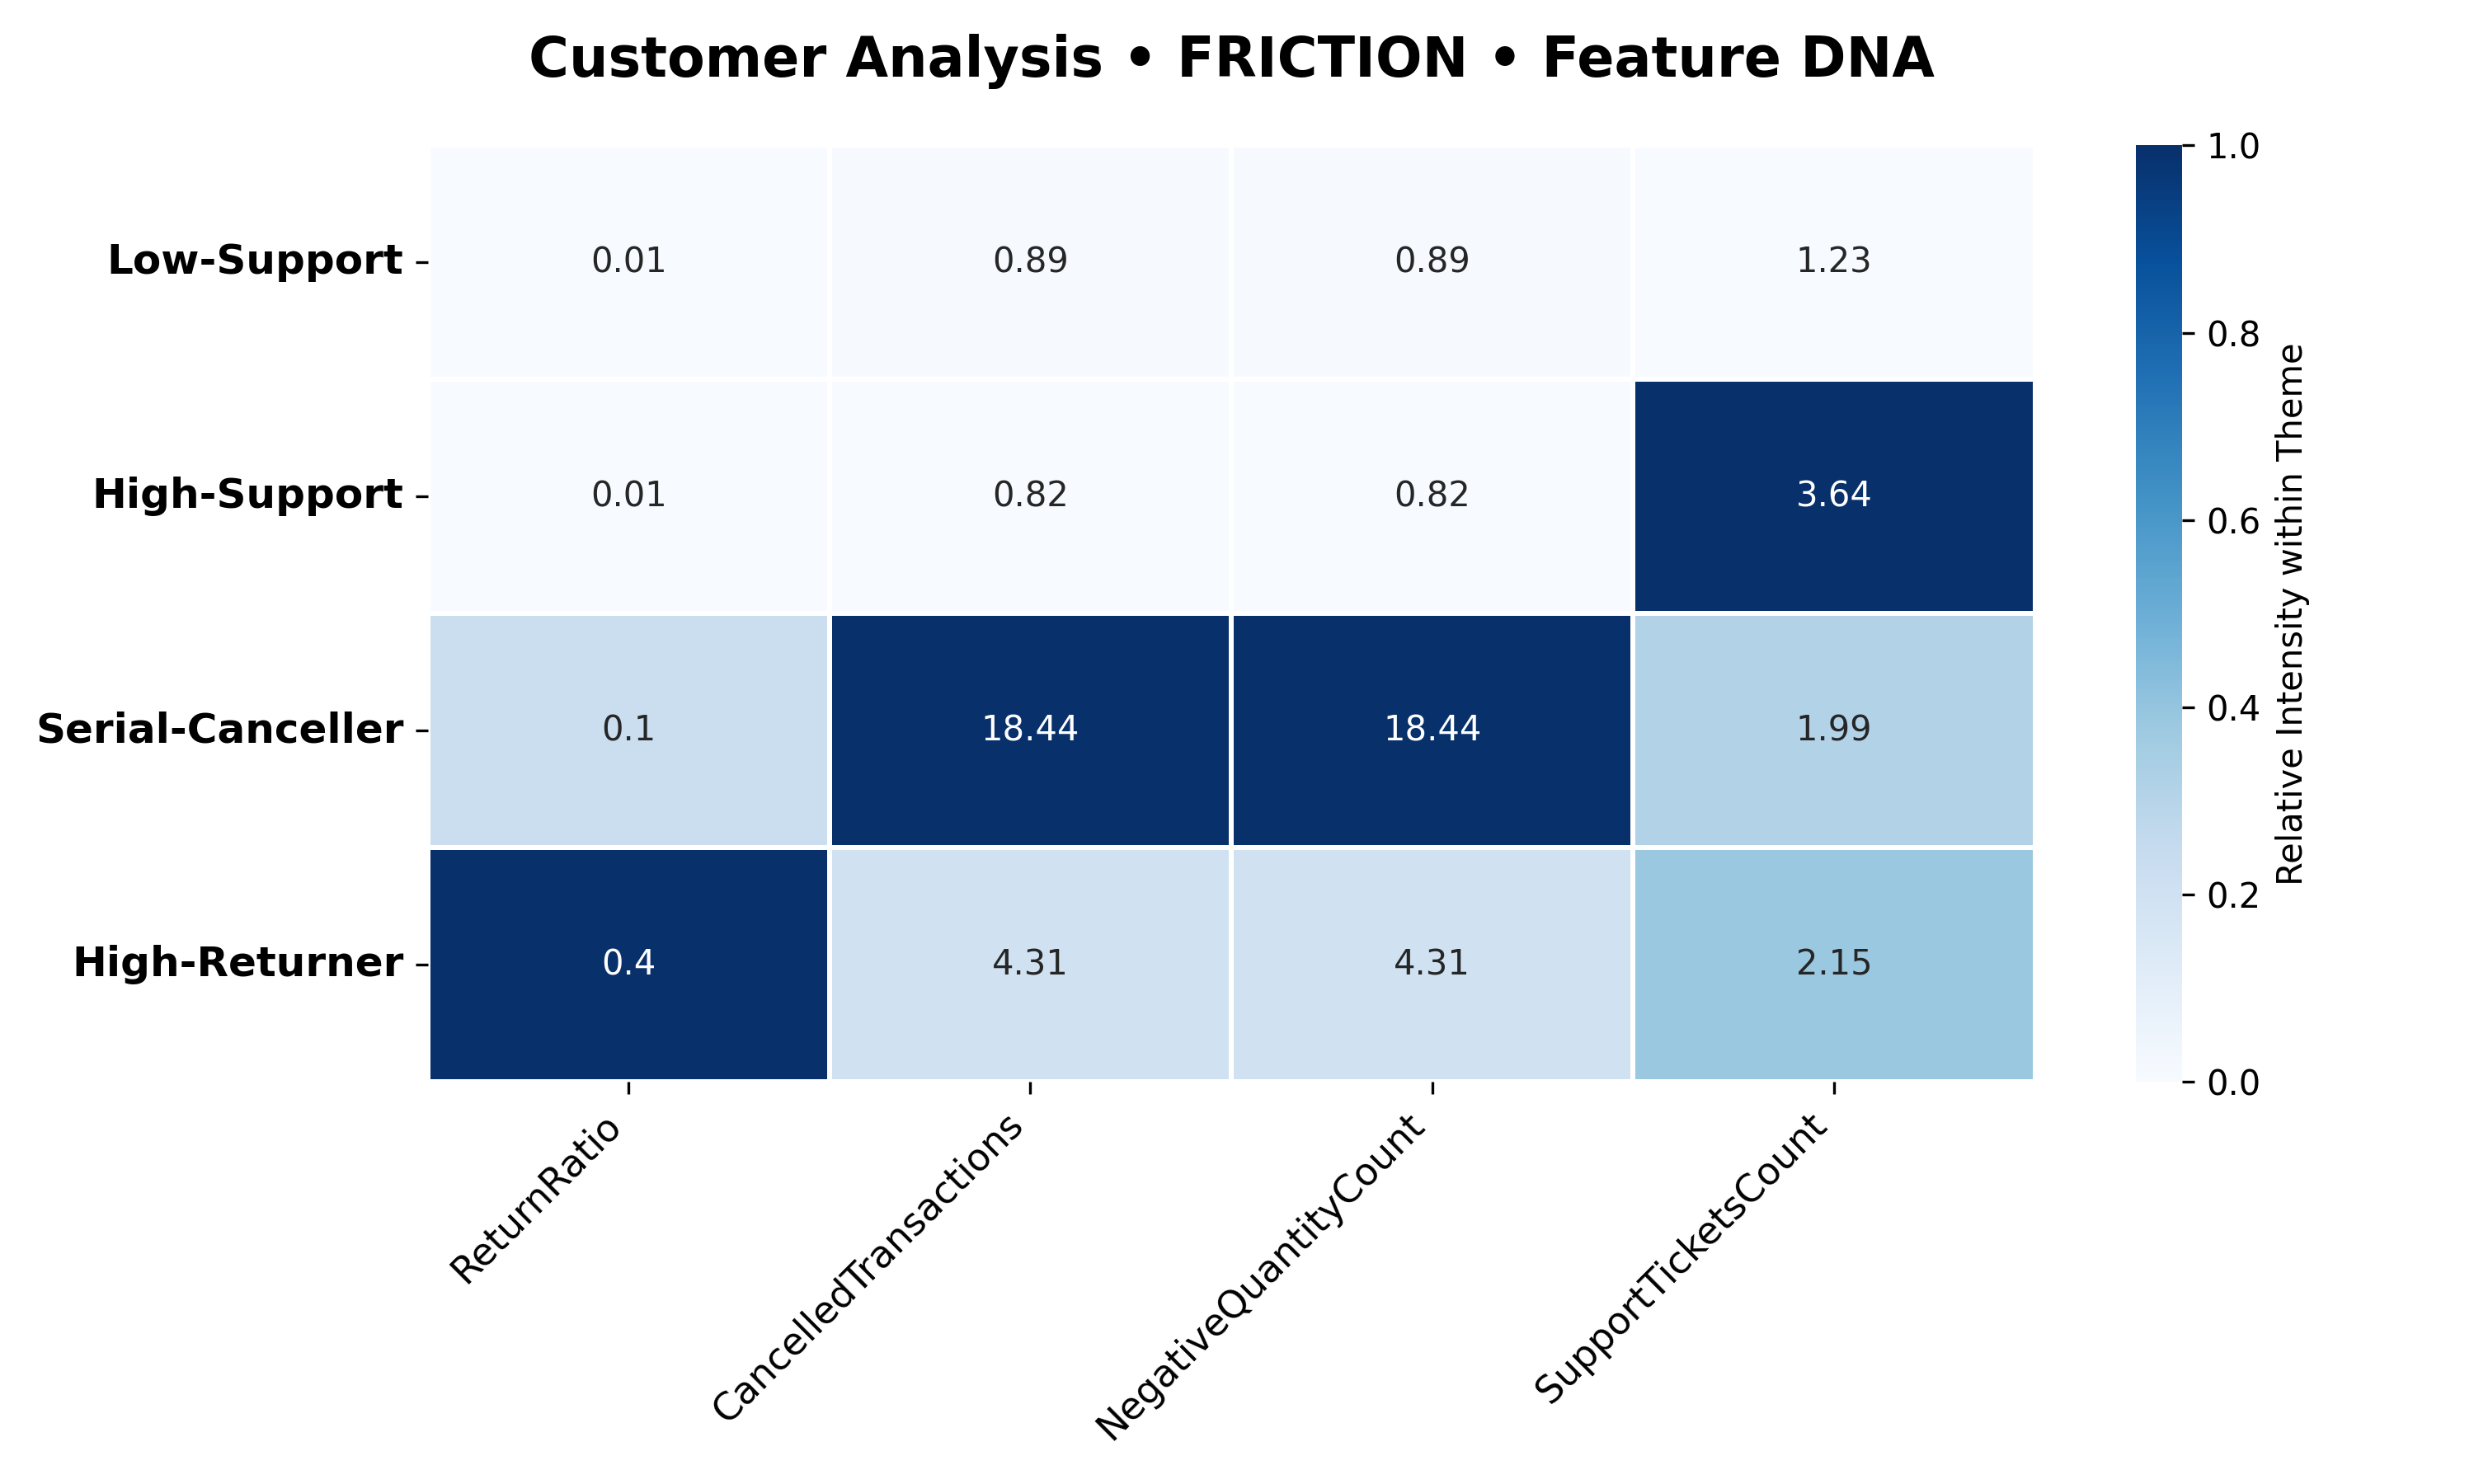
\includegraphics[width=0.75\textwidth]{figures/segmentation/friction_feature_heatmap.png}
    \caption{Friction Axis --- Feature importance heatmap per cluster.}
\end{figure}

\begin{figure}[H]
    \centering
    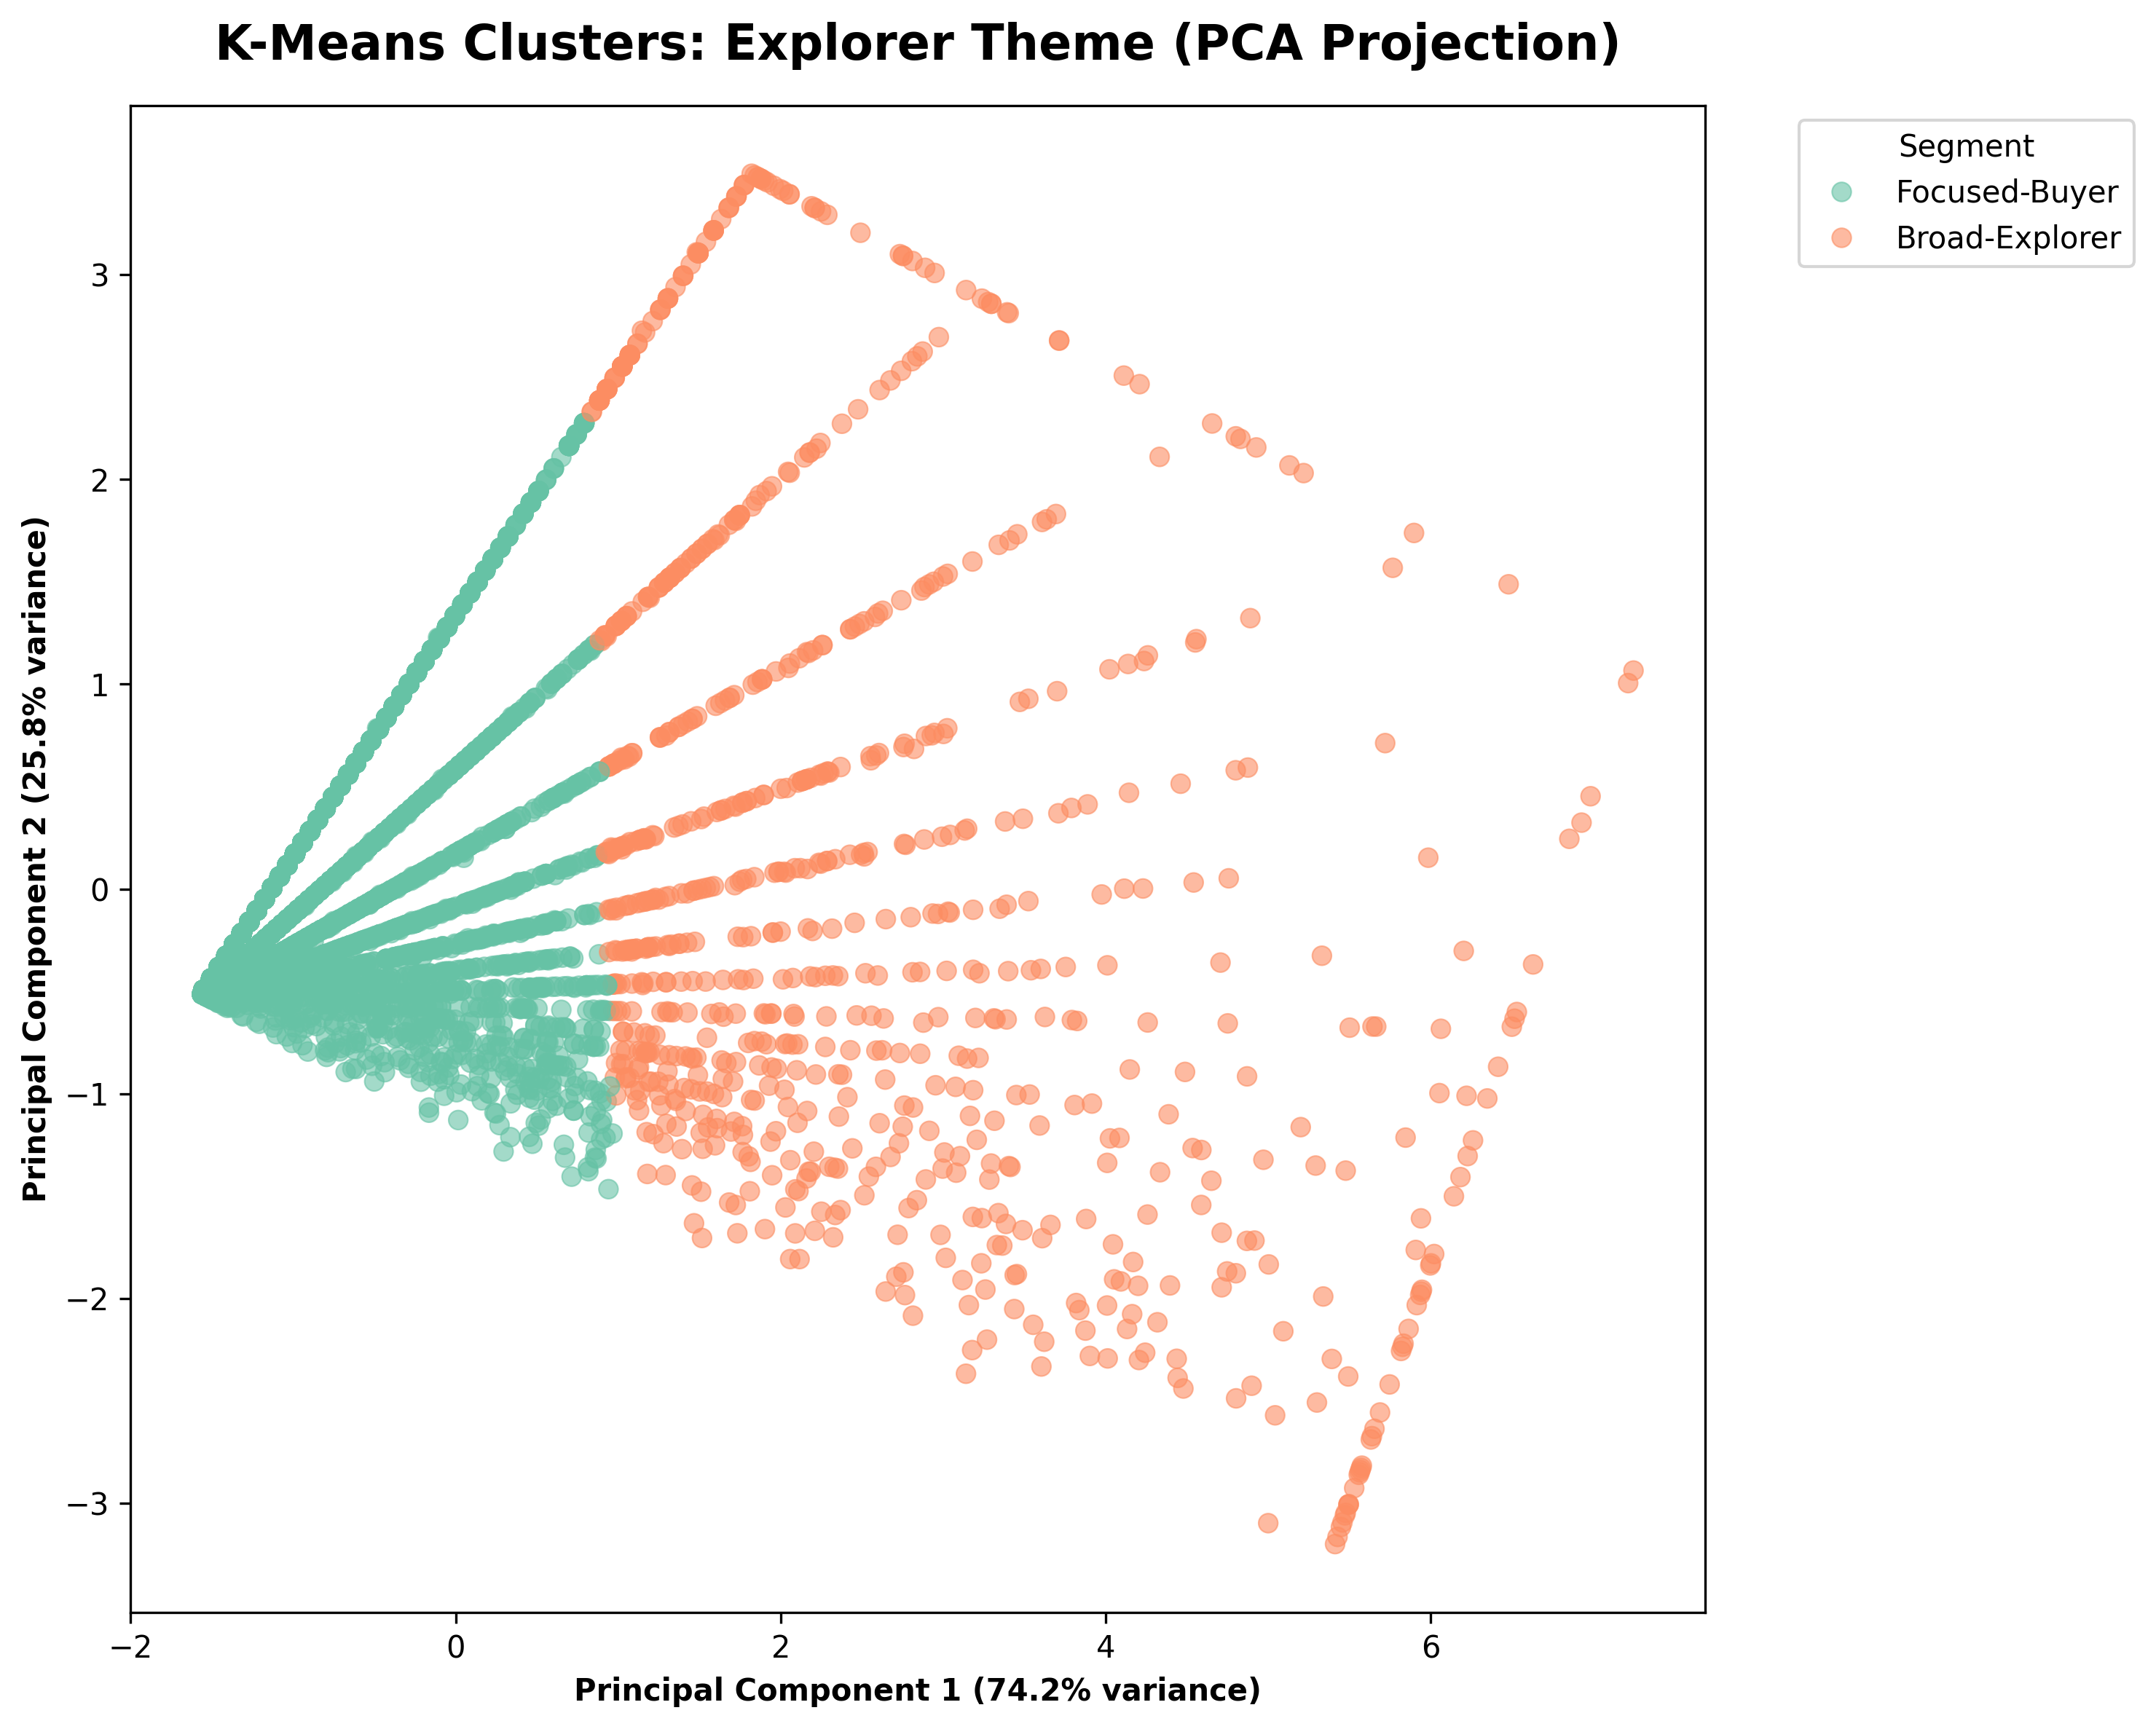
\includegraphics[width=0.9\textwidth]{figures/segmentation/explorer_kmeans_scatter.png}
    \caption{Explorer Axis --- Cluster scatter (PCA projection). Focused-Buyer, Broad-Explorer.}
    \label{fig:explorer_seg}
\end{figure}

\begin{figure}[H]
    \centering
    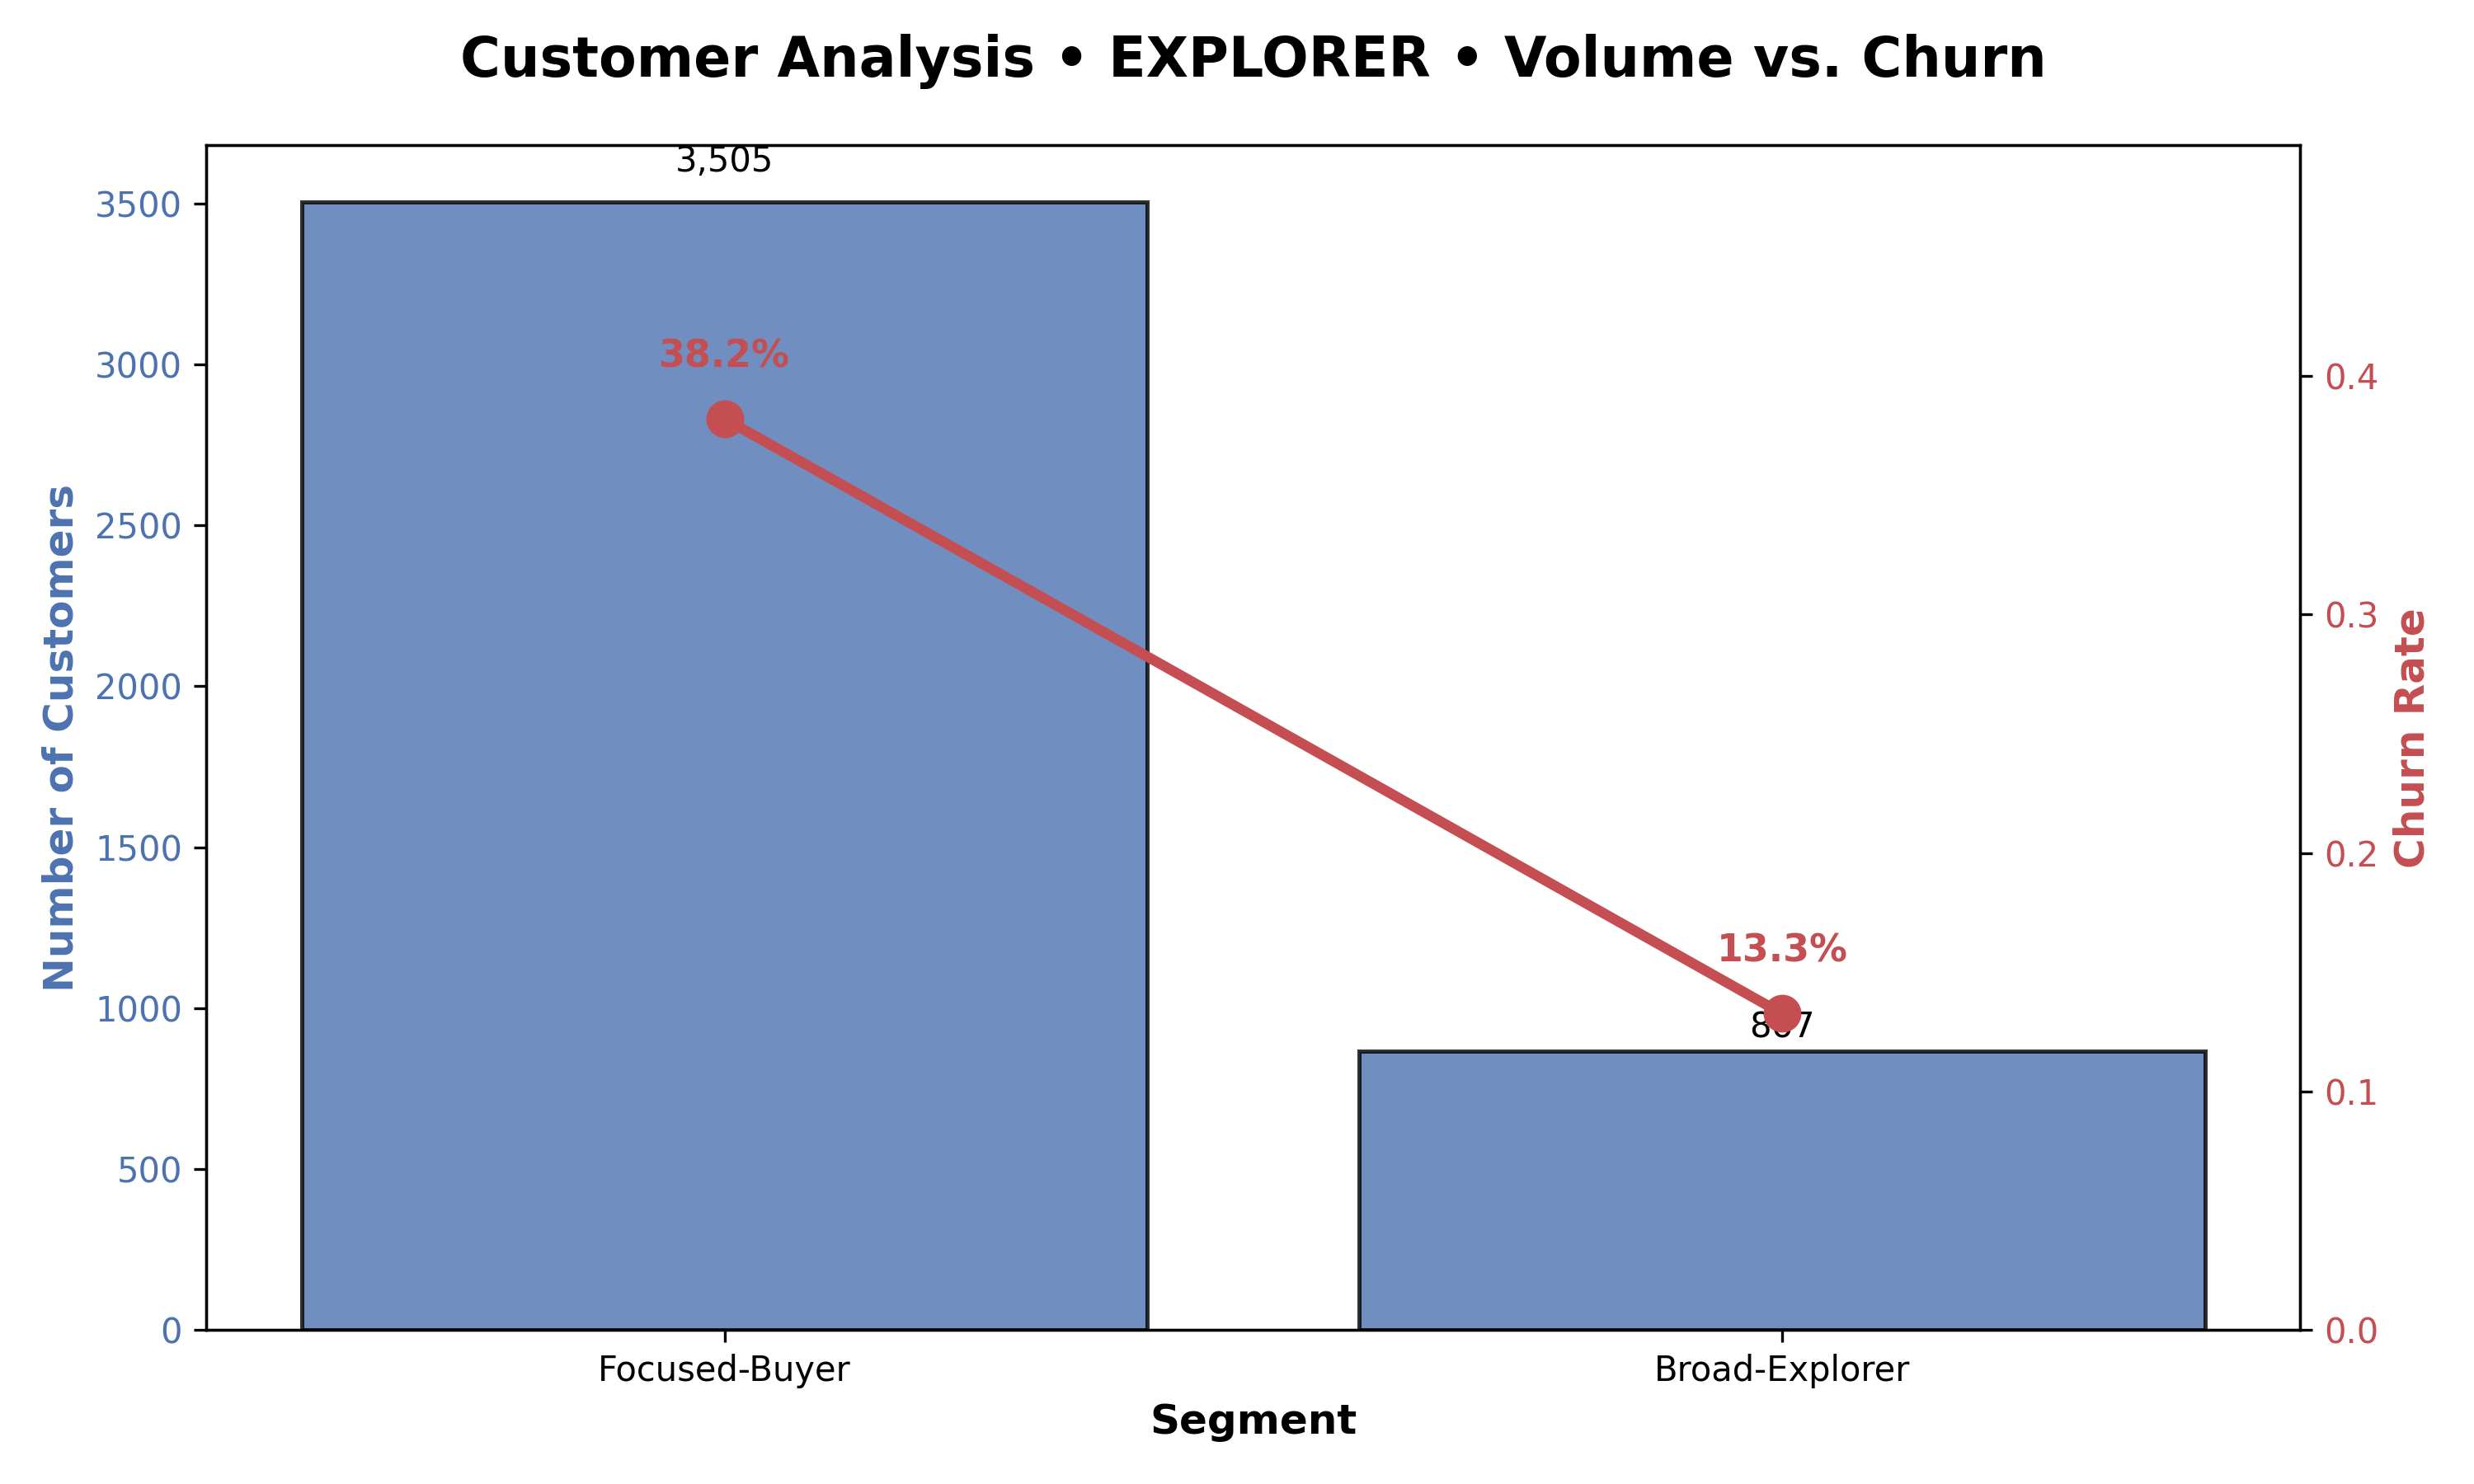
\includegraphics[width=0.75\textwidth]{figures/segmentation/explorer_size_vs_churn.png}
    \caption{Explorer Axis --- Cluster size vs. churn rate (Silhouette: 0.59).}
\end{figure}

\begin{figure}[H]
    \centering
    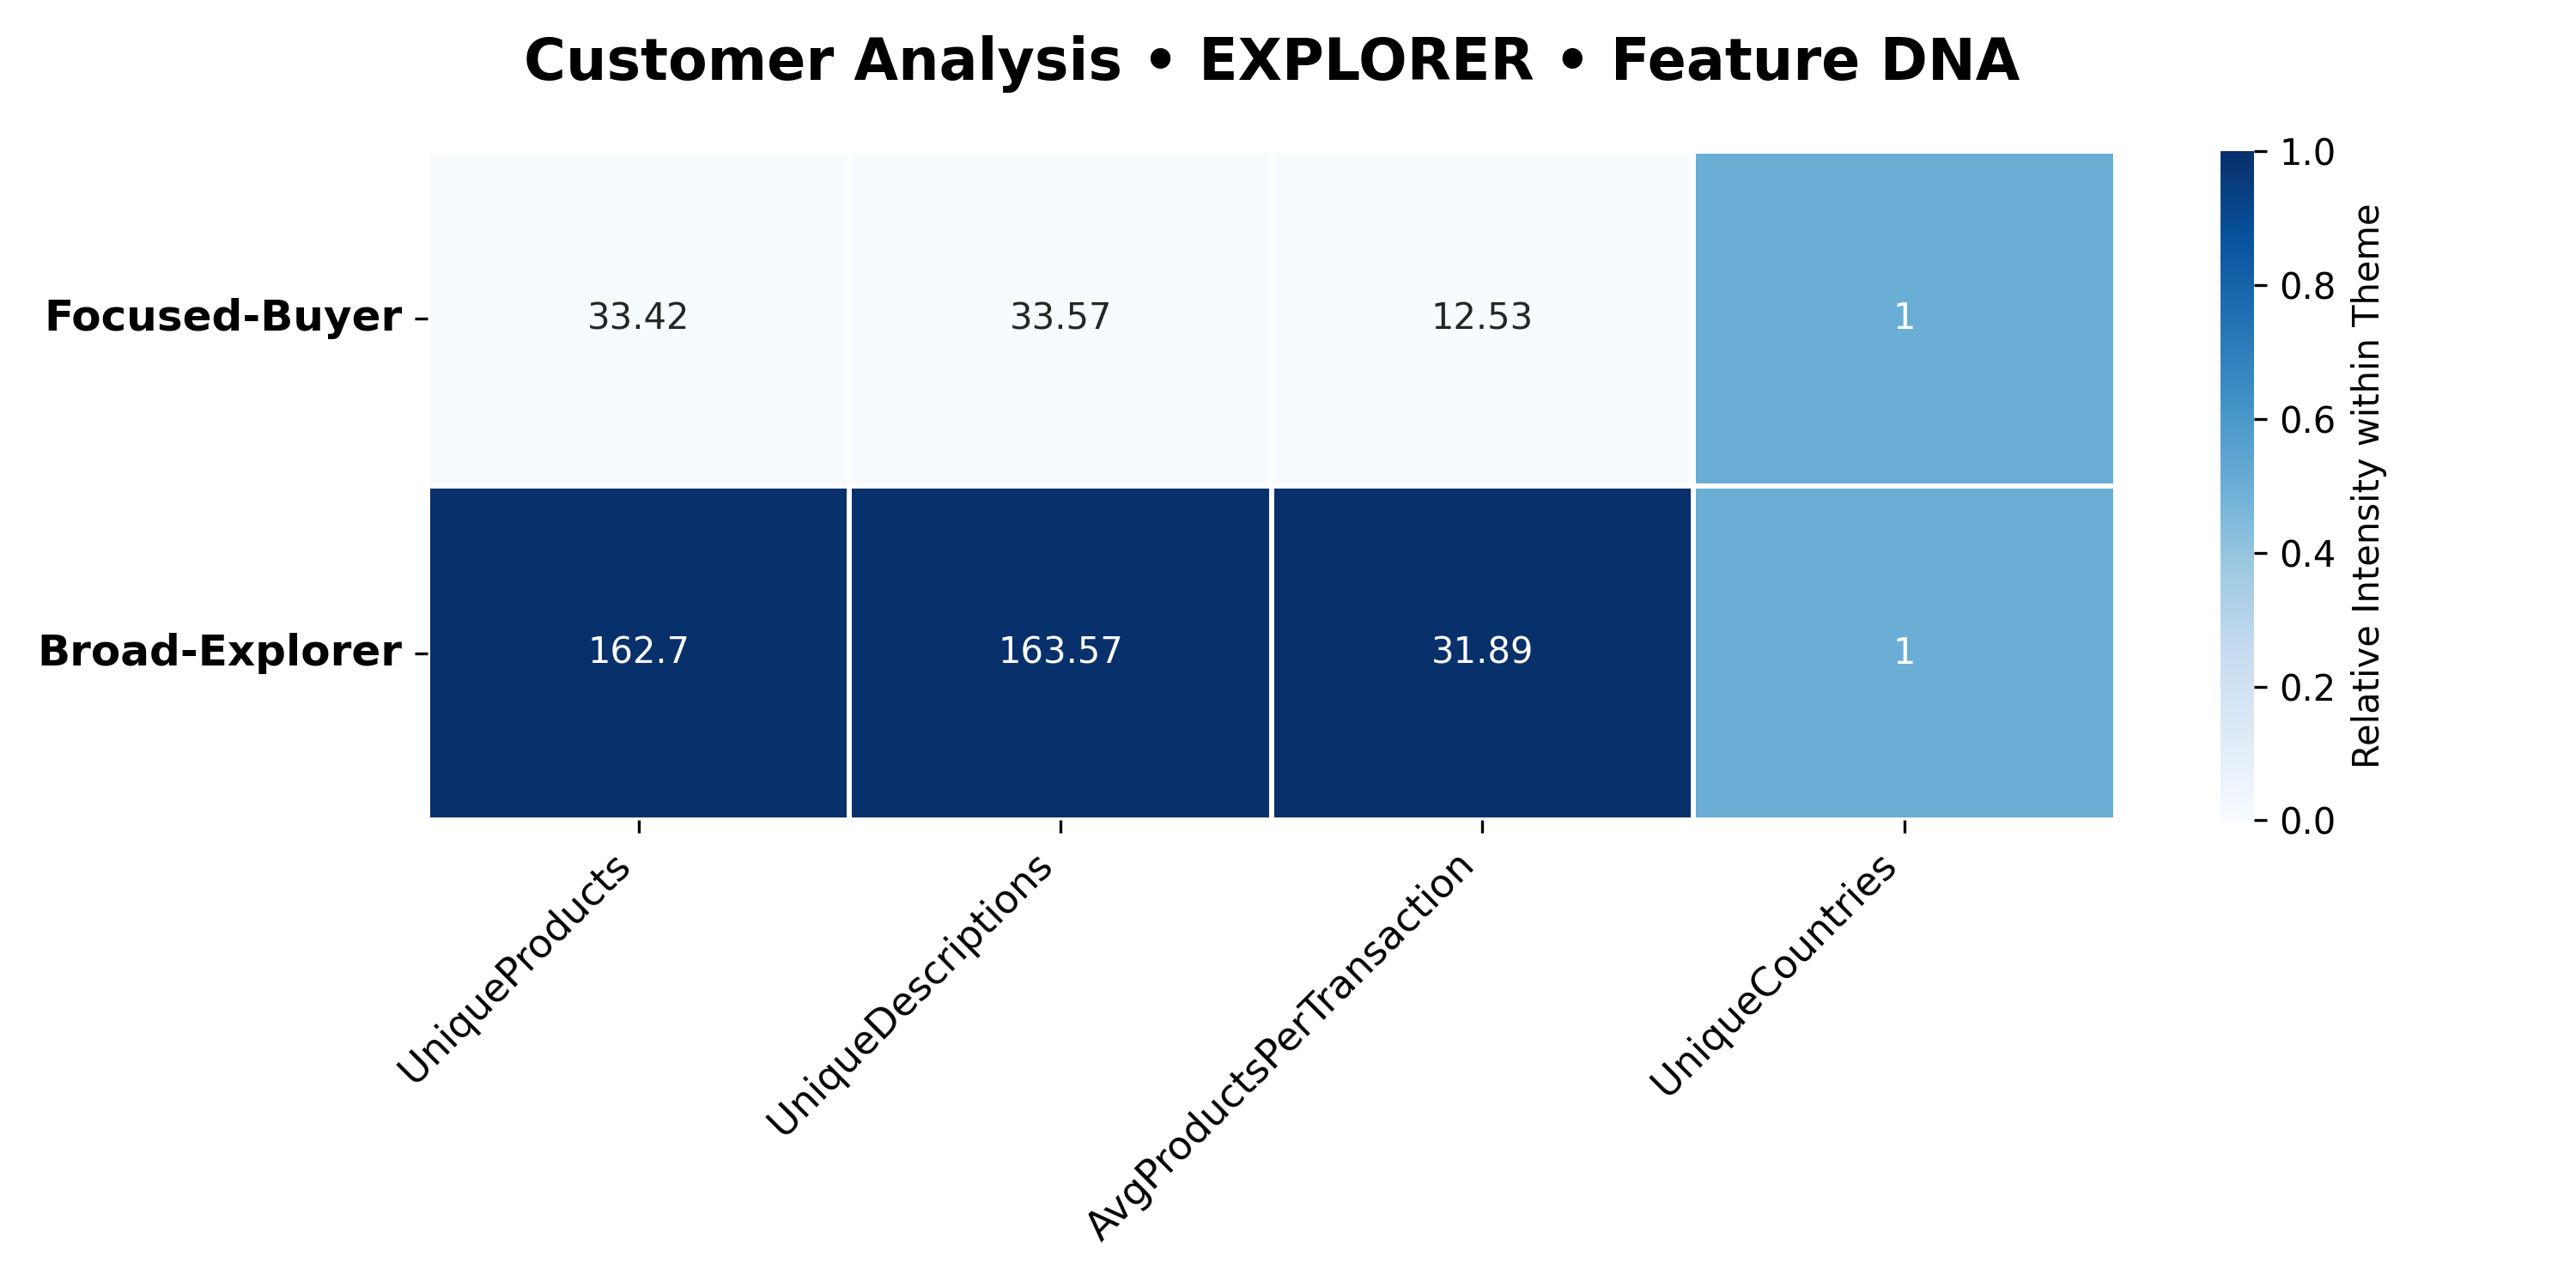
\includegraphics[width=0.75\textwidth]{figures/segmentation/explorer_feature_heatmap.png}
    \caption{Explorer Axis --- Feature importance heatmap per cluster.}
\end{figure}

\begin{figure}[H]
    \centering
    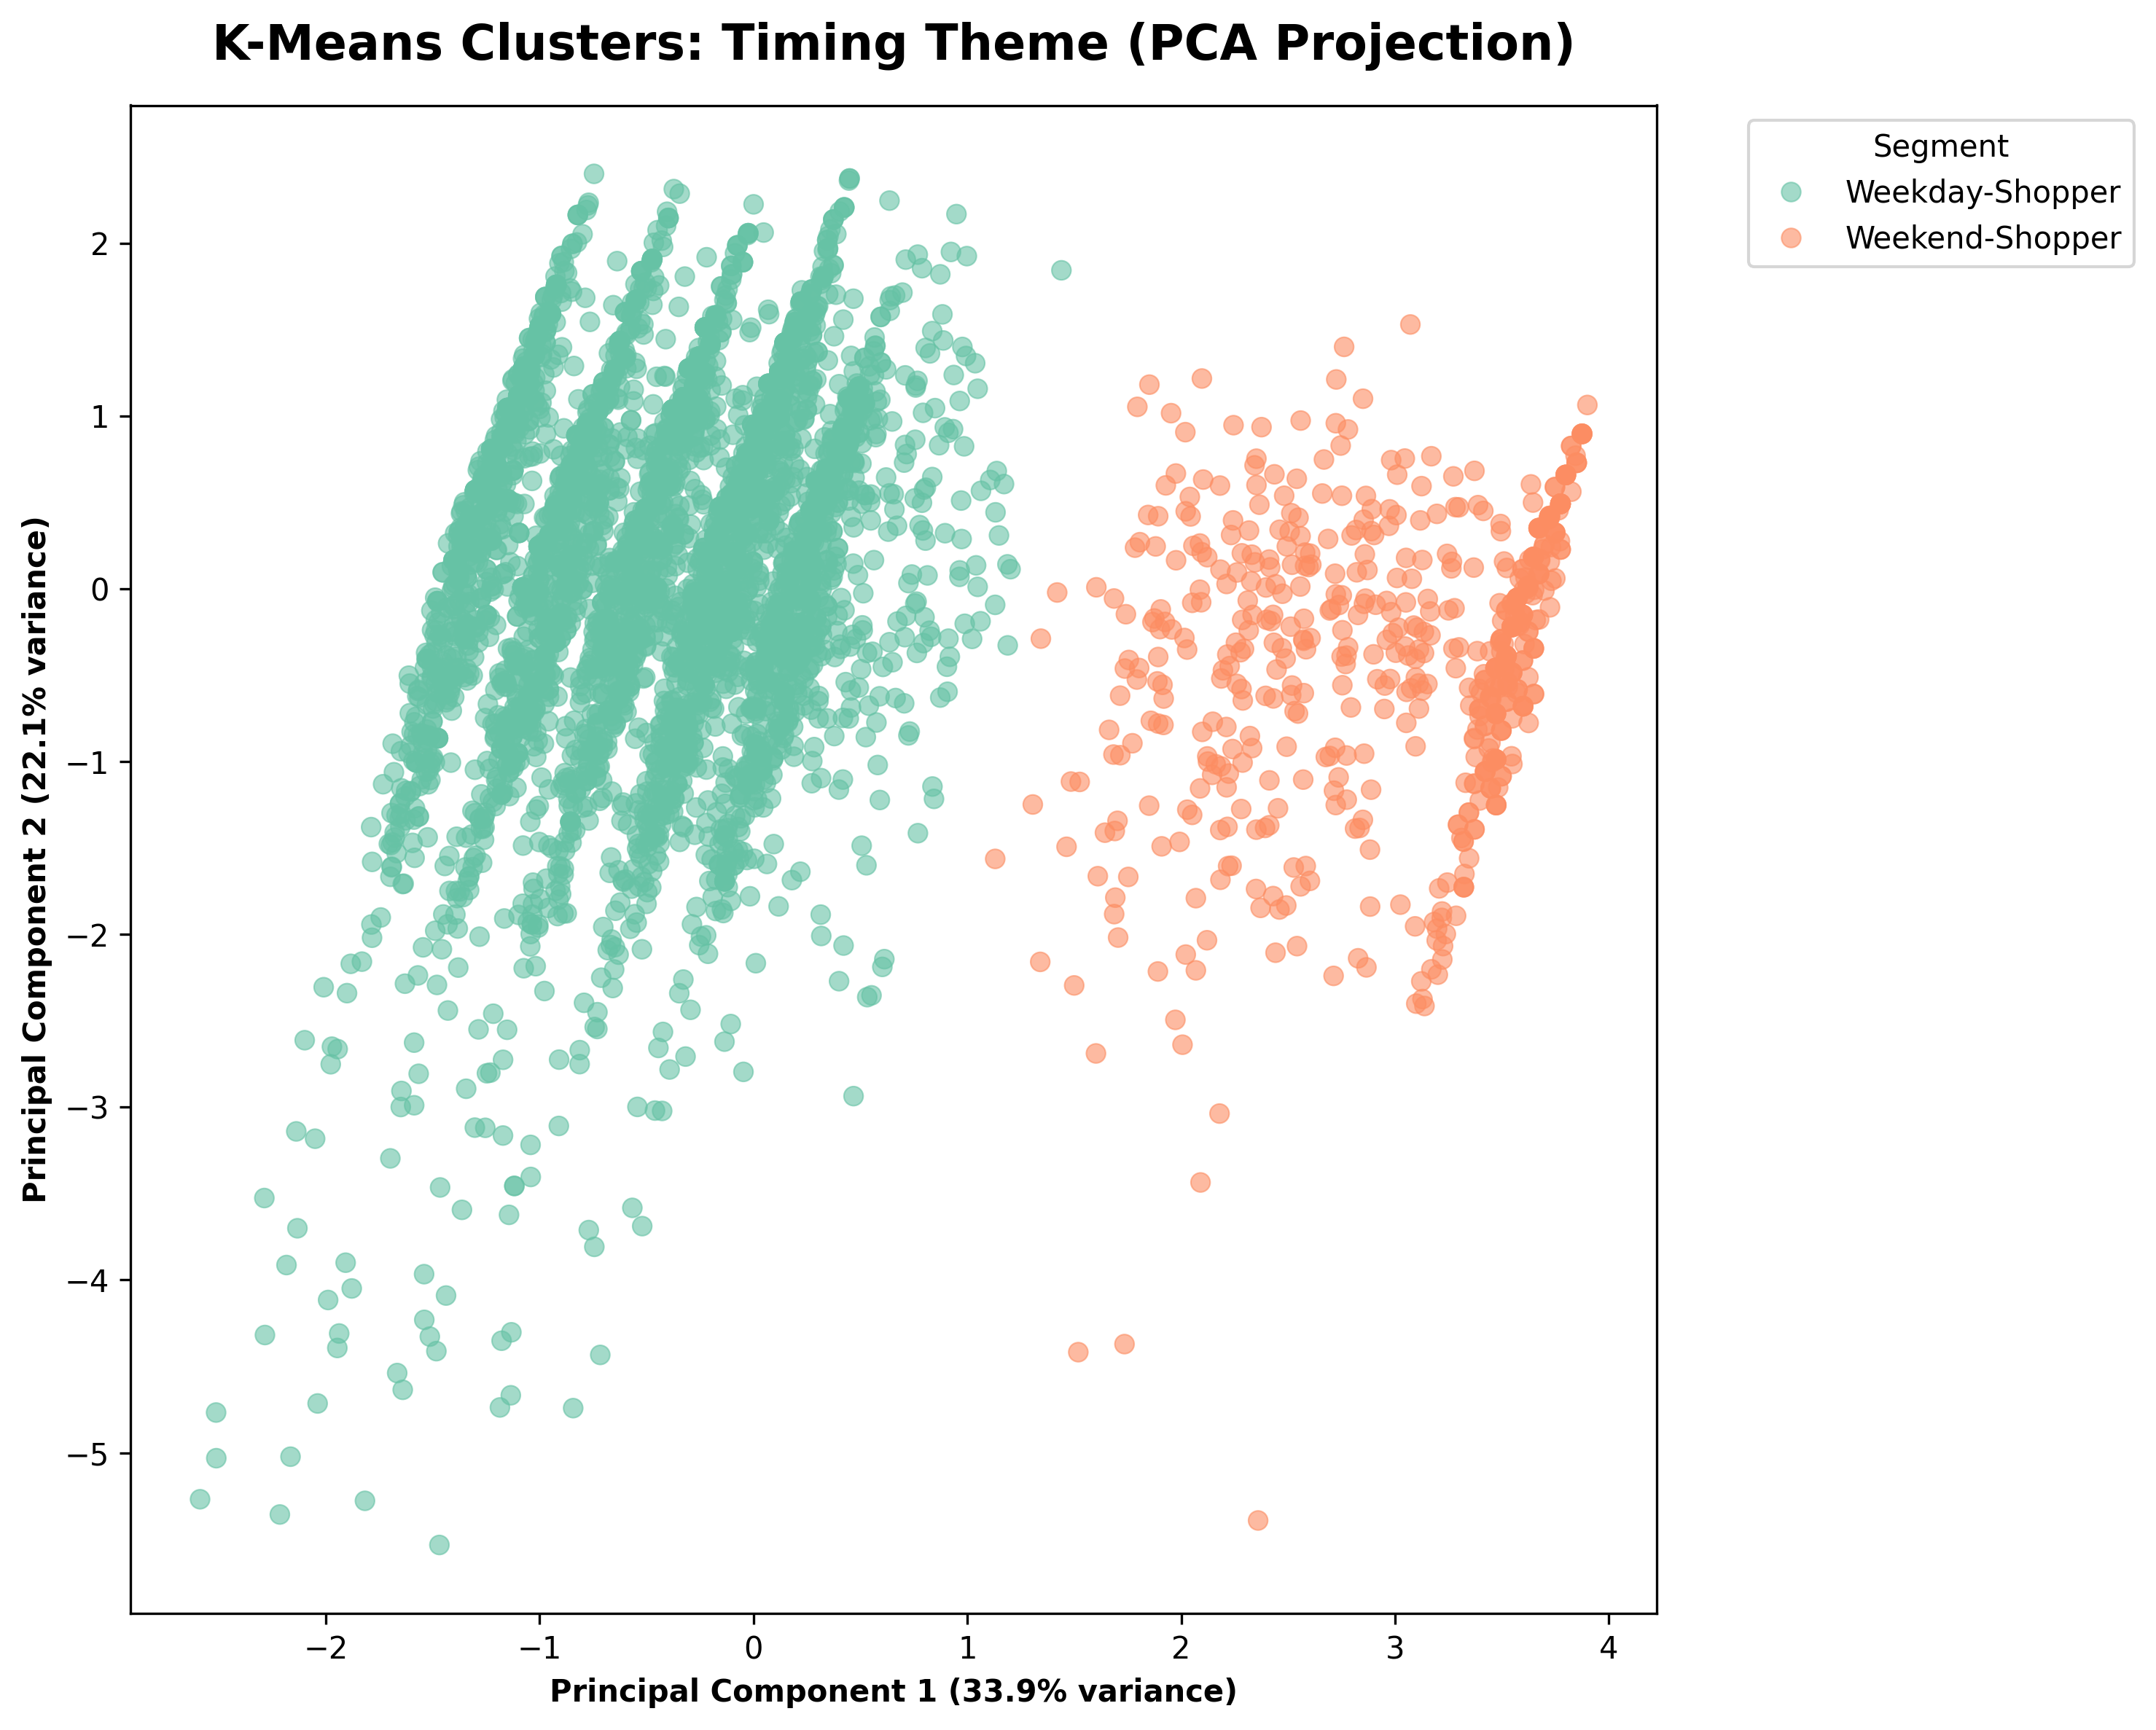
\includegraphics[width=0.9\textwidth]{figures/segmentation/timing_kmeans_scatter.png}
    \caption{Timing Axis --- Cluster scatter (PCA projection). Weekday-Shopper, Weekend-Shopper.}
    \label{fig:timing_seg}
\end{figure}

\begin{figure}[H]
    \centering
    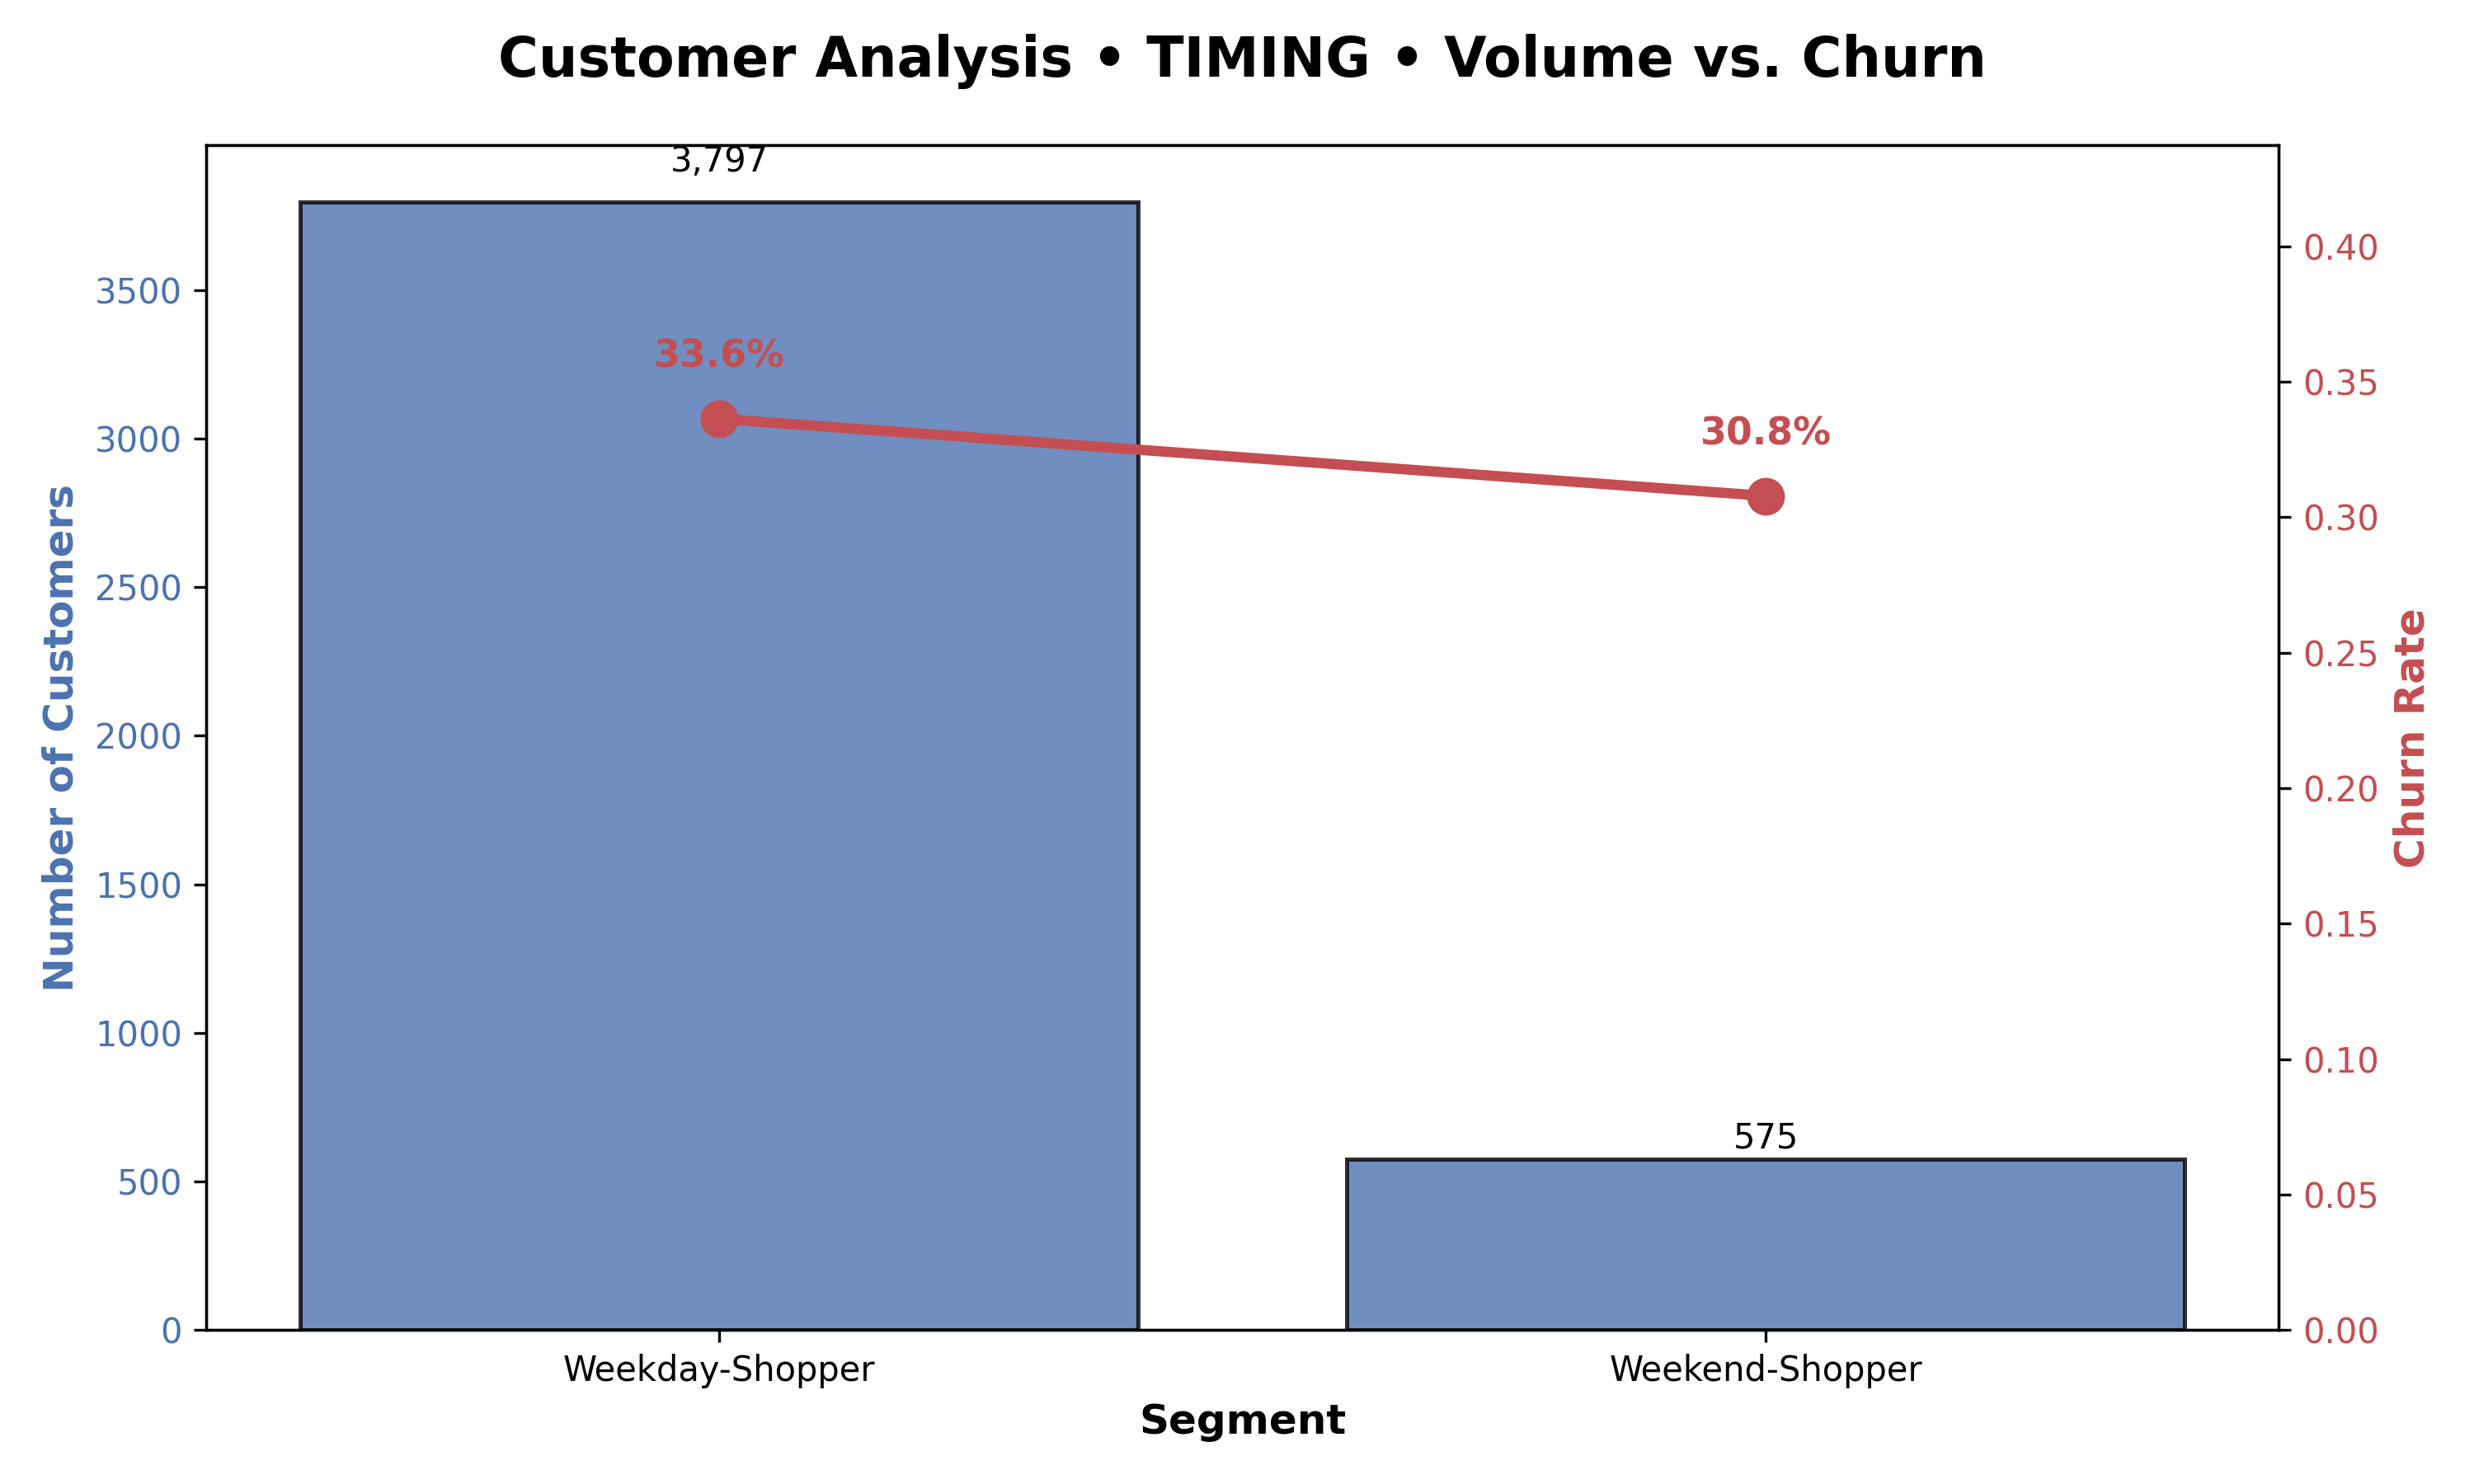
\includegraphics[width=0.75\textwidth]{figures/segmentation/timing_size_vs_churn.png}
    \caption{Timing Axis --- Cluster size vs. churn rate (Silhouette: 0.41).}
\end{figure}

\begin{figure}[H]
    \centering
    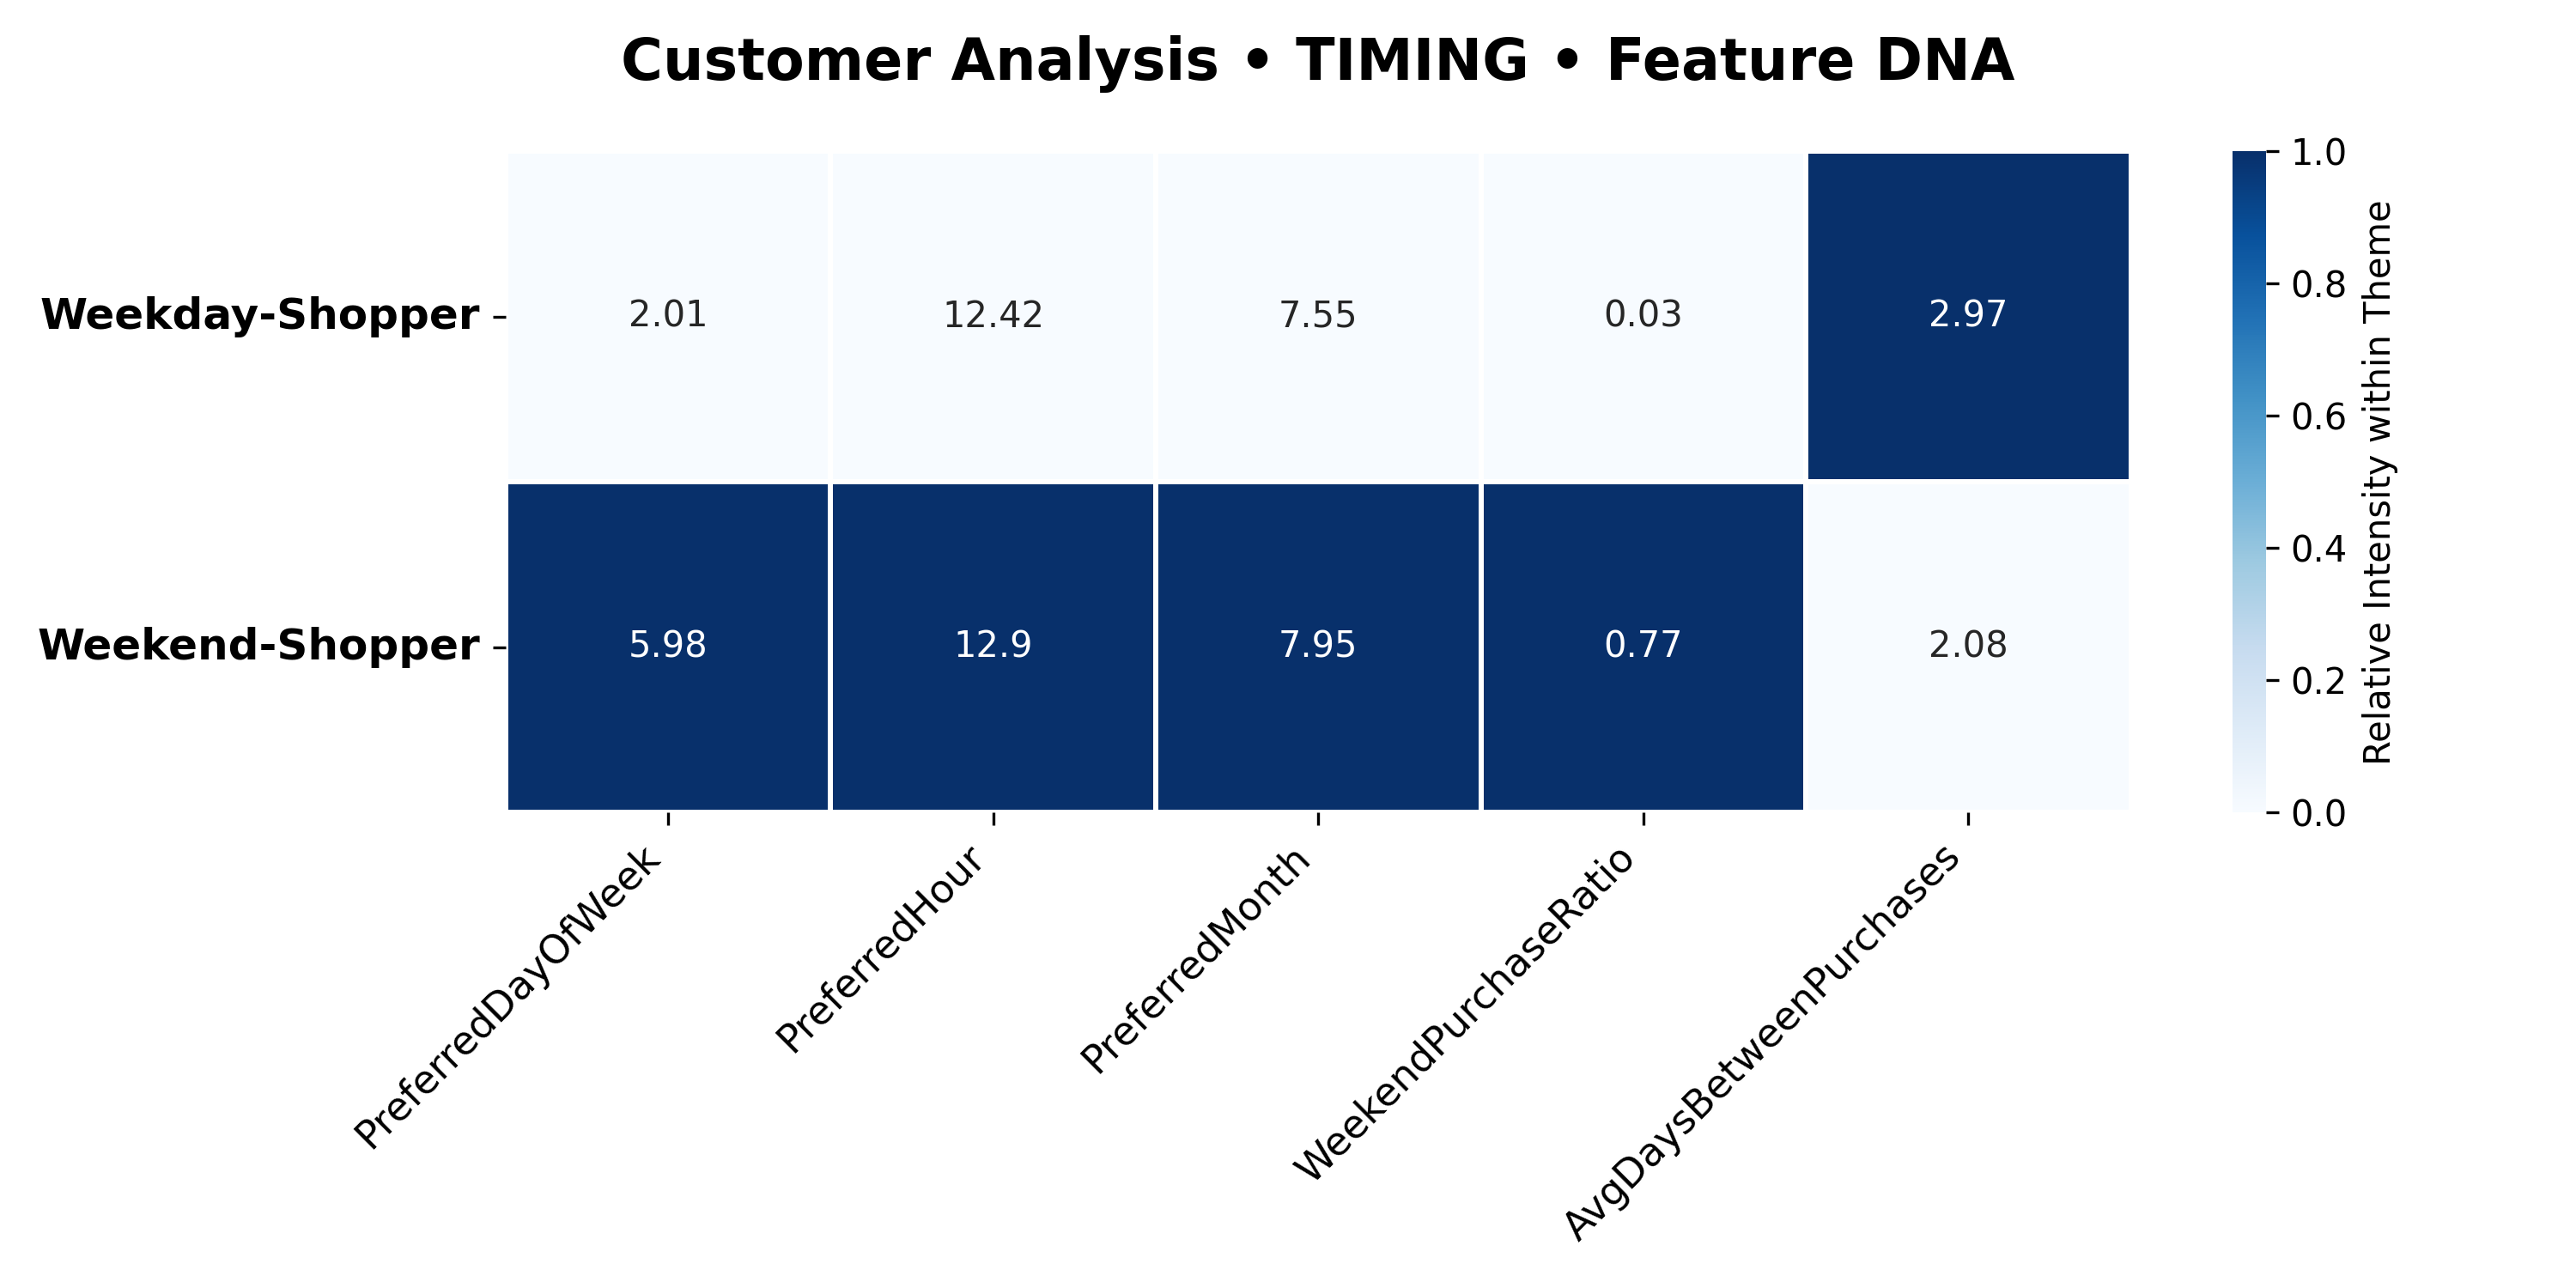
\includegraphics[width=0.75\textwidth]{figures/segmentation/timing_feature_heatmap.png}
    \caption{Timing Axis --- Feature importance heatmap per cluster.}
\end{figure}
\subsection{Classification Evaluation}

Metrics on the test set, notably the Area Under the ROC Curve (\textbf{AUC}) and overall accuracy, demonstrated excellent generalizing capability (see Figure~\ref{fig:roc_curves}). Specifically, the models achieved the following test accuracies: \textbf{Random Forest} (94.29\%), \textbf{Logistic Regression} (98.74\%), \textbf{Gradient Boosting} (96.00\%), and \textbf{XGBoost} (96.00\%). 

Optimization led to selecting \textbf{XGBoost} as the final reference model due to its robust accuracy (96.00\%) and superior precision/recall ratio on the critical prediction (the leaving customer). Confusion matrices enabled business collaborators to estimate the impacts of false negatives (undetected lost customers), as visualized in Figure~\ref{fig:confusion_matrix}.

\begin{figure}[H]
    \centering
    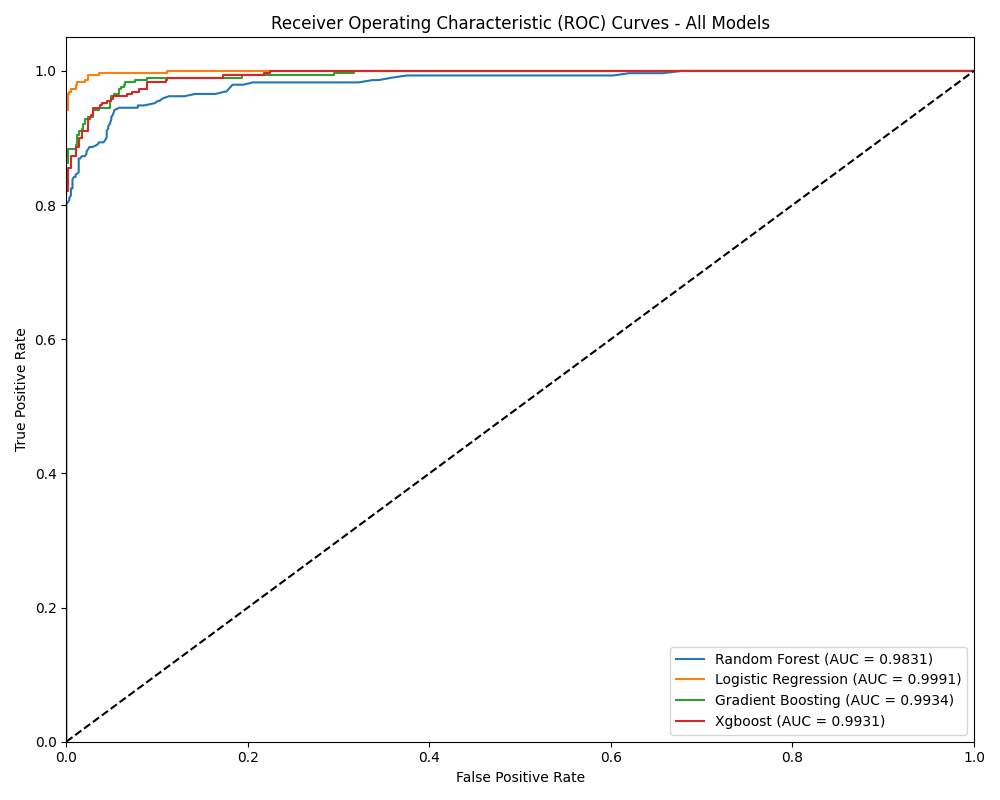
\includegraphics[width=0.55\textwidth]{figures/modeling/roc_curves_combined.png}
    \caption{ROC-AUC Curves for all evaluated models.}
    \label{fig:roc_curves}
\end{figure}

\begin{figure}[H]
    \centering
    \begin{subfigure}{0.48\textwidth}
        \centering
        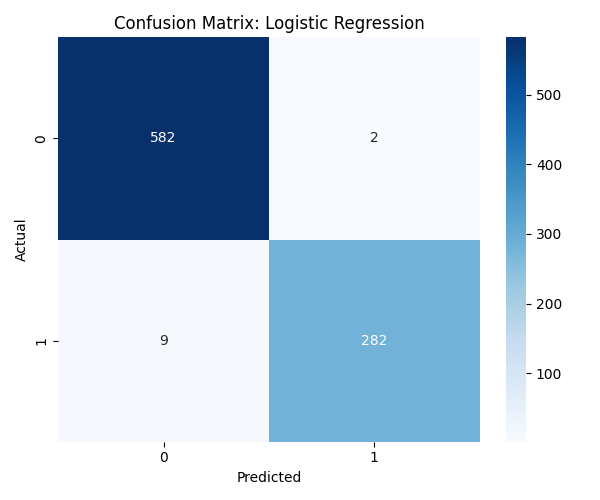
\includegraphics[width=\linewidth]{figures/modeling/logistic_regression_confusion_matrix.png}
        \caption{Logistic Regression}
    \end{subfigure}
    \hfill
    \begin{subfigure}{0.48\textwidth}
        \centering
        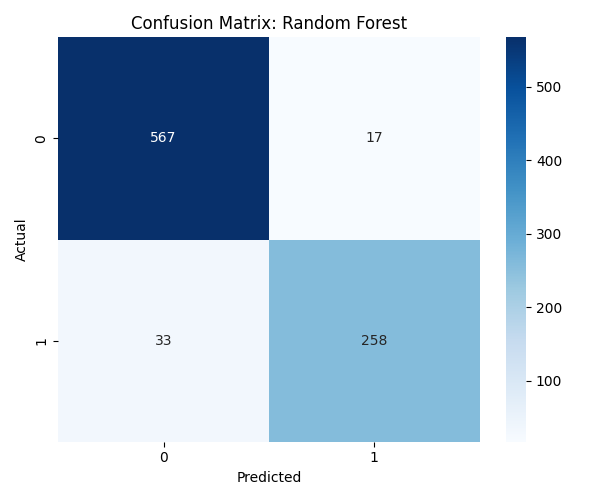
\includegraphics[width=\linewidth]{figures/modeling/random_forest_confusion_matrix.png}
        \caption{Random Forest}
    \end{subfigure}
    
    \vspace{0.4cm}
    \begin{subfigure}{0.48\textwidth}
        \centering
        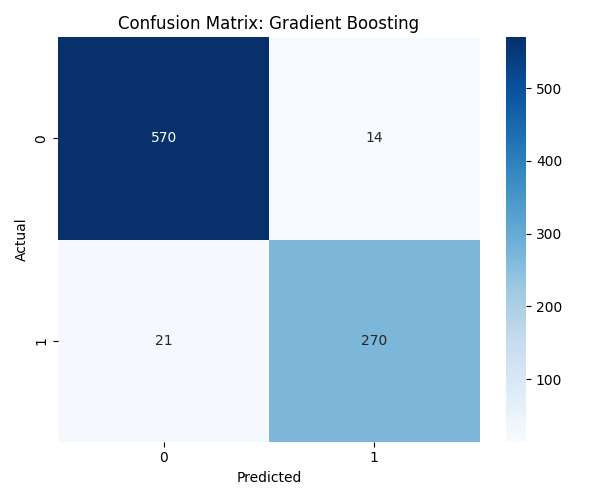
\includegraphics[width=\linewidth]{figures/modeling/gradient_boosting_confusion_matrix.png}
        \caption{Gradient Boosting}
    \end{subfigure}
    \hfill
    \begin{subfigure}{0.48\textwidth}
        \centering
        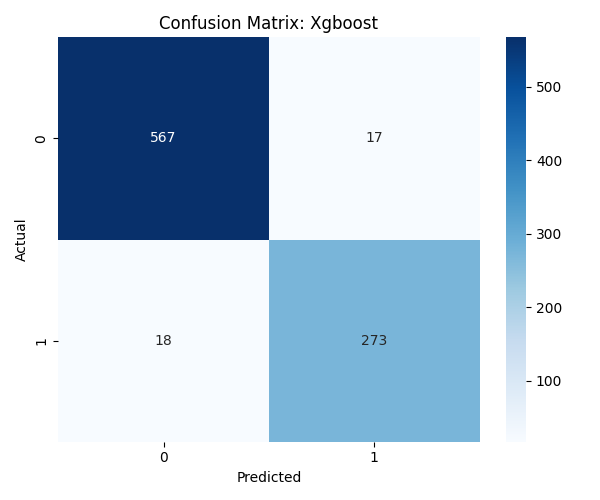
\includegraphics[width=\linewidth]{figures/modeling/xgboost_confusion_matrix.png}
        \caption{XGBoost}
    \end{subfigure}
    \caption{Confusion Matrices for all evaluated models: (a) Baseline Linear, (b) \& (c) Ensemble frameworks, and (d) the final top-performing XGBoost architecture.}
    \label{fig:confusion_matrix}
\end{figure}

\section{Deployment}

In compliance with the culmination of the CRISP-DM life cycle, the technical phase was materialized into a robust web application. Built with \textbf{Flask}, it enables exposing:
\begin{itemize}
    \item \textbf{A dynamic front-end}: Customer test forms are generated via the interface strictly aligning with the initial feature profiling (via the \texttt{/api/schema} endpoint).
    \item \textbf{Instant Demo Sampling}: An \texttt{/api/sample} endpoint was explicitly programmed to instantly fetch and stream a fully randomized pre-processed customer profile directly into the UI.
    \item \textbf{Real-time inference}: The complete preparation pipeline (\textit{fitted transformers}, scalers, and PCA generated during training) is instantiated on new data and the \textbf{XGBoost} model is called.
    \item \textbf{Behavioral Profiling}: The application does not merely return the final churn risk probability; it explicitly maps and displays the user's computed segment categorizations across the 3 core thematic axes (\textit{Friction}, \textit{Explorer}, and \textit{Timing}) to provide immediate contextual depth alongside the prediction.
\end{itemize}

\begin{figure}[H]
    \centering
    \begin{subfigure}{0.68\textwidth}
        \centering
        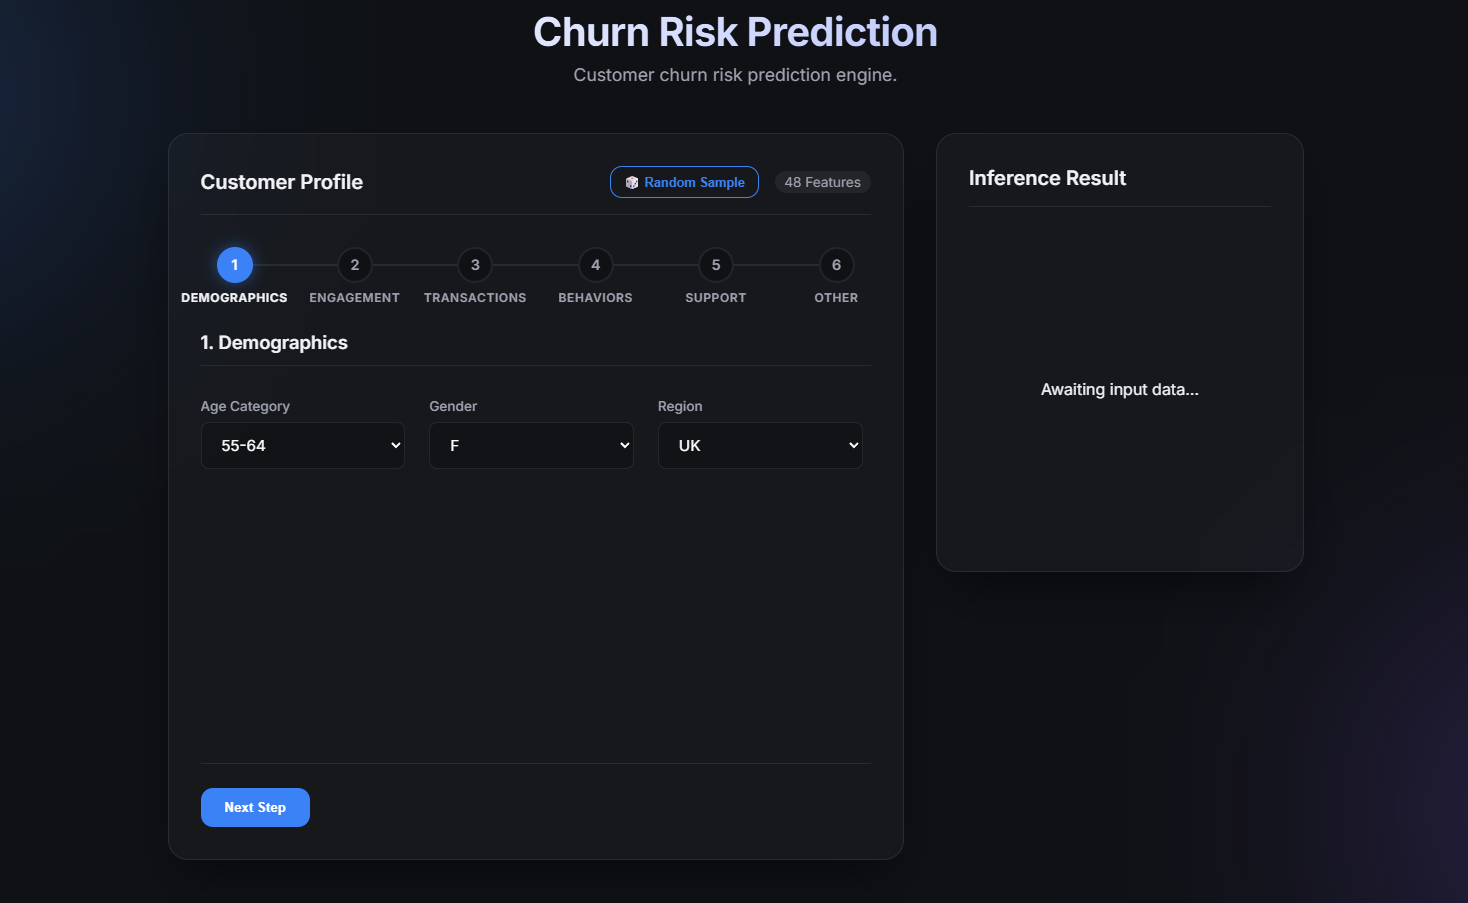
\includegraphics[height=6.5cm, keepaspectratio]{figures/deployment/hs.png}
        \caption{Flask Application Homescreen}
    \end{subfigure}%
    \hfill
    \begin{subfigure}{0.28\textwidth}
        \centering
        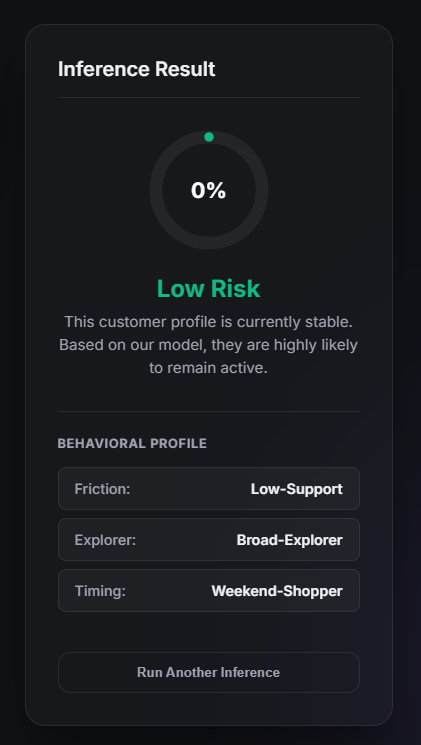
\includegraphics[height=6.5cm, keepaspectratio]{figures/deployment/result.png}
        \caption{Real-Time Inference Result Panel}
    \end{subfigure}
    \caption{Deployment Interface: Submitting a customer profile for live XGBoost churn prediction and segment profiling.}
    \label{fig:deployment}
\end{figure}

\section{Conclusion}

By restructuring traditional customer analysis through the full implementation of the Data Science lifecycle, this project shifts from simple descriptive interpretation of raw data to a predictive, interactive, and business-focused system. The combination of K-Means profiling by "themes" and XGBoost Churn prediction now equips the company for surgical marketing campaigns and optimized retention.

\end{document}